%!TEX root = ../PhDthesis.tex
\chapter{Literature Review}

The field of neuroscience has experienced an explosion in the size,
quantity and quality of data being collected over the past few
decades, but over the same time period very few novel theoretical
advances have been made. Most of our theories for how the brain
operates have been left unchanged by the radical improvements in
techniques such as optogenetics and two-photon calcium imaging. A
major obstacle to converting these breakthroughs in experimental
neuroscience to genuine advances in our theoretical understanding of
the brain is the difficulty in relating the many individual
observations into a coherent picture of how these circuits work.

This problem is particularly evident in visual neuroscience, one of
the most extensively researched areas in neuroscience, due to the
relative ease with which the visual areas can be accessed, stimulated
and studied. Since the first models of the function of the visual
system were developed by the pioneers of visual neuroscience, namely
Mountcastle and Hubel and Wiesel we have collected tremendous amounts
of data and developed models to explain particular phenomena. However,
we have made very little progress on explaining the fundamental
computations performed in visual cortical areas; most of the core
ideas such as receptive and association fields have been around since
the early pioneers proposed them.

In this thesis we will argue that this failure to make significant
advances in understanding the computations performed by the visual
system is primarily a failure to attempt to integrate our knowledge
across various levels of description. This issue is precisely what
David Marr highlighted when stating that the brain, and the visual
system in particular, should be analyzed at three distinct but
complementary levels of analysis \citep{Marr1982}, later expanded to
include a fourth level by Tomaso Poggio \citep{Poggio2012}. According
to Marr and Poggio, models of cognitive systems such as the mammalian
visual system should describe the system at one or more of the
following levels of analysis:

\begin{itemize}
\item Learning: How does the system learn to perform the necessary
  computations?
\item Computational: What does the system actually do? What
  computations does it perform?
\item Algorithmic/Representational: How does the system represent the
  problem and solve it?
\item Implementational/Physical: How is the system physically
  implemented?
\end{itemize}

Each of these levels of evidence when viewed in isolation can
contribute to the overall understanding about the system, but to gain
real insights, models should begin abstracting across these levels of
analysis to find out where and how evidence from various sources fit
together (or more interestingly, highlight potential
discrepancies). In this chapter we will summarize the current
knowledge about the circuits, cell classes and functions performed by
the primary visual cortex at each of these levels before starting to
integrate that information into models that will allow us to make
novel predictions about the physical implementation, algorithmic
operation, and computational function as well as learning and
development.  We will begin by reviewing the anatomy and physiology of
the early visual system.

\section{Early Visual System: Areas and layers}

The earliest stage of the mammalian visual system (pictured in
Figure~\ref{VisualSystem}) is the retina, where rod and cone
photoreceptors convert incident photons into electrical and chemical
signals. These signals are then further converted from analogue
voltages into spike trains by retinal bipolar and ganglion cells and
sent down the optic nerve to the lateral geniculate nucleus
(LGN). Connections from the two eyes cross over at the optic chiasm to
form projections of the right and left visual field
contra-laterally. The connections from the retina map retinotopically
onto the LGN, meaning that nearby areas of the LGN respond to nearby
portions of the visual field. After the initial processing in the
retina and LGN, the visual stream is projected onto the primary visual
cortex (V1).

\begin{figure}
	\centering
        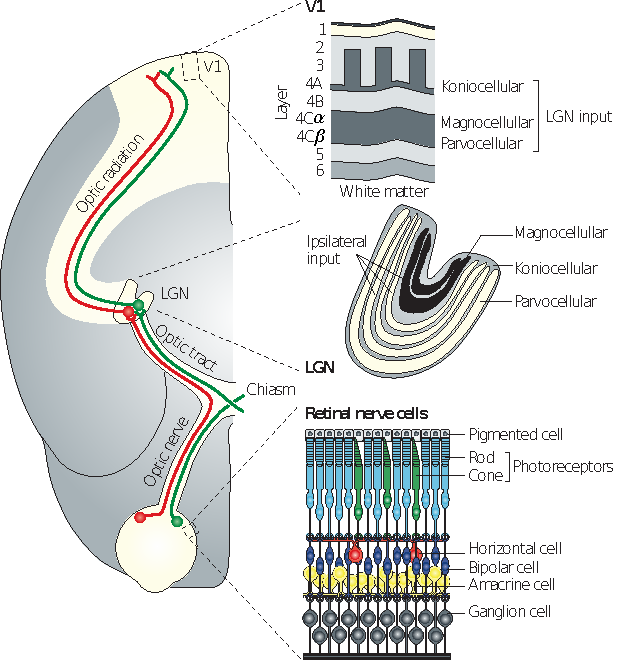
\includegraphics[width=0.9\textwidth]{solomon.pdf}
	\caption[A diagram of the early visual pathway in mammals, reproduced
      from \cite{Solomon2007}.]{The early visual pathway in primates
      (also generally the same for most other mammals) from
      the retina to the primary visual cortex (V1) via the lateral
      geniculate nucleus (LGN) of the thalamus. The left panel shows
      the pathway, while the right panels highlight noteworthy
      sections including the structure of the retina, with the LGN and V1
      broken down into their different layers and showing different
      cell types. Adapted from \cite{Solomon2007}.}
	\label{VisualSystem}
\end{figure}

In the retina, summation of various photoreceptor types gives rise to
so called center-surround receptive fields. These ON- and OFF-center
receptive fields can arise in bipolar cells but are more commonly
associated with retinal ganglion cells (RGCs). This receptive field
type responds most strongly to spots of light/dark moving through the
visual field (as shown in Figure~\ref{Center-Surround}) but can be
characterized as simple edge detectors.

\begin{figure}
	\centering 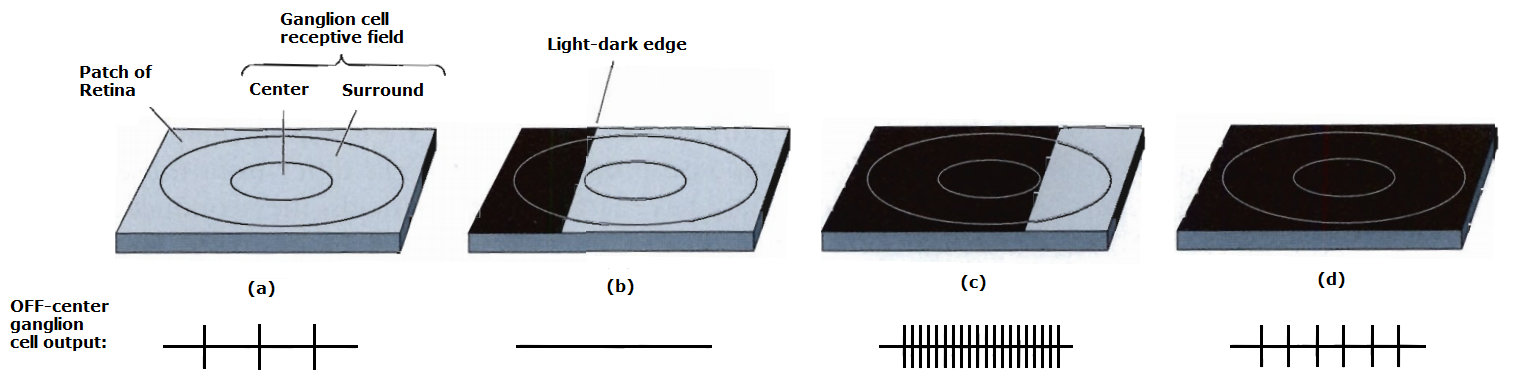
\includegraphics[width=0.9\textwidth]{Figure2.png}
	\caption[A Center-surround receptive field. Adapted from
      \cite{Bear2006}.]{The center-surround receptive field structure
      of some retinal ganglion cells and LGN neurons, illustrating how
      a contrast edge activates different portions of the field and
      thereby results in different activation patterns. From left to
      right one can see that as the light-dark edge moves into the ON
      surround field, spontaneous activity is suppressed, and as it
      moves further over the OFF-center field the neuron becomes
      highly active. Adapted from \cite{Bear2006}.}
	\label{Center-Surround}
\end{figure}

In addition to the macro-organization of the visual system into
distinct areas, the LGN and downstream structures are further
broken down into individual layers and cell classes. The separation of
LGN cells into layers also corresponds to functional separations, as
layers 1, 4 and 6 usually receive contra-lateral input, while layers
2, 3 and 5 receive ipsi-lateral inputs from the retina. Furthermore,
different layers consist of different cell types, with ventral layers
1 and 2 containing larger so called magno-cellular (M) neurons and
dorsal layers 3, 4, 5 and 6 containing smaller parvo-cellular (P)
neurons with intra-laminar neurons being referred to as konio-cellular
(K). Since these three cell types are also present in the retina and
make connections mainly with their own cell type it is theorized that
each carries its own parallel information stream. Functionally,
P-cells have displayed greater sensitivity to chromatic contrast and
higher spatial frequencies, linking them to the processing of detail
and color, while M-cells have been shown to have greater sensitivity
for high temporal frequencies associating them with motion processing.

\subsection{Primary Visual Cortex: Topographic Maps, Simple and Complex Cells}

The primary visual cortex (V1) or striate cortex provides the first
cortical stage of processing of visual information. The cortex was
classically divided into six layers but since then several subdivisions have
been added after functional sub-groups were discovered. Feedforward
input from the LGN is received in layer 4C$\alpha$ and 4C$\beta$ ,
which receive input most of their input from M- and P-cells
respectively. The neurons in layer 4 then send projections up to
layers 2/3, which has a diverse intra-laminar network of connections
but also sends intracortical projections to a number of higher visual
areas, while layers 5 and 6 provide feedback to the LGN.

Neurons in the primary visual cortex (V1) are tuned to respond to a
variety of different features or complex combinations of such
features, including orientation, spatial and temporal frequency,
motion direction, color or ocular origin. In many mammalian species,
including primates and carnivorans, these feature preferences map
smoothly and topographically onto the cortical surface. This mapping
extends vertically through the layers of the cortex, giving rise to
the notion of distinct cortical columns. Retinotopy arises due to the
mapping of visual information straight from the retina to the LGN and
then to the cortex. Other response preferences such as orientation and
direction selectivity rarely arise in primate LGN and are usually thought
of as emergent phenomena in the cortex.

% jbednar: any particular reason to use ferret rather than macaque
% here, given that all of your thesis is about macaque?  It doesn't
% much matter, but e.g. Blasdel '92 would be less surprising here.
\begin{figure}
	\centering 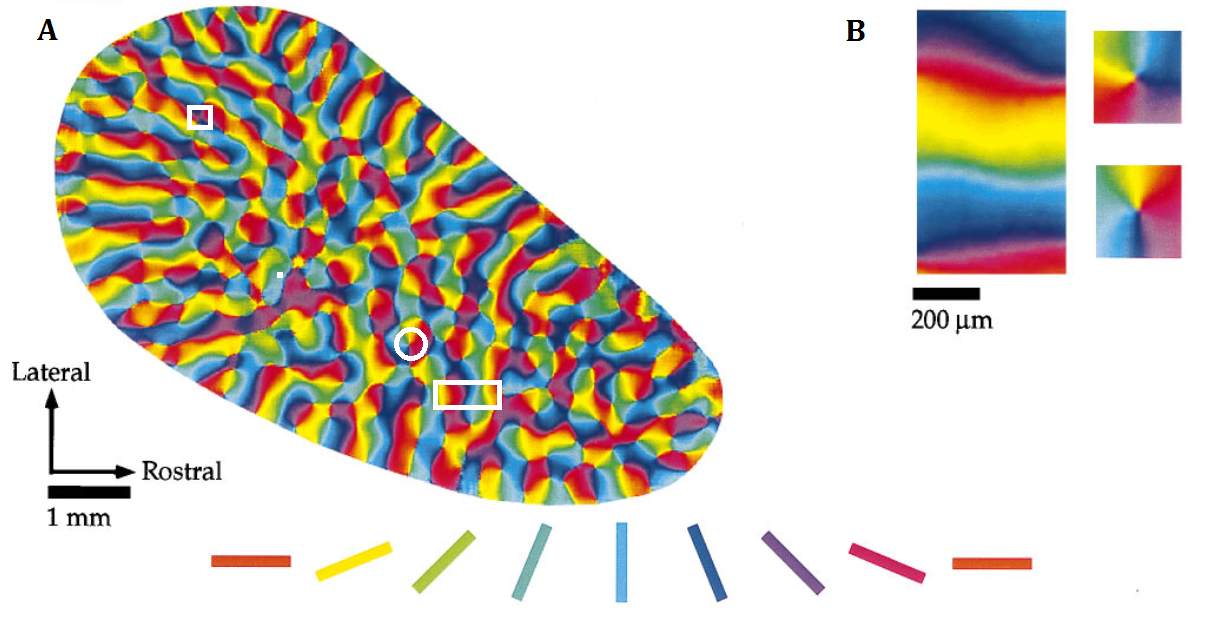
\includegraphics[width=0.9\textwidth]{Figure3.png}
	\caption[A ferret orientation map in primary visual
      cortex. Adapted from \cite{Bosking1997}.]{A) Orientation
      preference map in ferret V1 generated by overlaying the activity
      maps for different orientations and artificially coloring each
      area according to the orientation preference using the color key
      below. The image also highlights three common features
      of orientation maps in white. The square highlights a saddle
      point, where a patch of cortex selective for a particular
      direction is almost bisected by a patch selective to another
      direction. The circle highlights a pinwheel arrangement, where
      different orientations preference patches are arranged in a
      circular shape. Finally the rectangular shape highlights a
      linear zone in which orientation preference change
      continuously. B) Magnifications of a linear zone and two
      pinwheel arrangements. Adapted from \cite{Bosking1997}.}
	\label{OrientationMap}
\end{figure}

The receptive fields of V1 neurons are different in that often there are no
longer simple ON- or OFF-center surround fields, forming more complex
spatio-temporal patterns. They are commonly modeled using Gabor filters
as shown in Figure~\ref{Gabor}, which have elongated ON and OFF
regions or lobes, generated by localizing a full-field sine grating
by multiplying it with a Gaussian envelope. Orientation selectivity and spatial
frequency preference are determined by the orientation and spacing of
ON- and OFF-regions respectively. It is also possible for V1 cells to
filter temporal patterns by employing spatio-temporal shifts in their
ON and OFF lobes, giving rise to direction selectivity.

Orientation-selective neurons can generally be classed as simple or
complex cells, depending on whether they display some form of
spatial/phase invariance \citep{Skottun1991}. In reality this
classification is not particularly clear, with cells being somewhere
on a gradient from pure simple cells to a complex cell with the degree
of phase invariance being the determining factor. Apart from phase
invariance the neurons often exhibit contrast invariance, such that
even at very low contrast they will respond more strongly to their
preferred orientation than to the orthogonal orientation
\citep{Sclar1982}.

\begin{figure}
	\centering 
\includegraphics[width=0.25\textwidth]{gabor.png}
        
\includegraphics[width=0.25\textwidth]{gabor90.png}
	\caption[Oriented Gabor patches.]{Gabor Patches at 0 degree and
      90/180 degree orientations with clearly visible ON (white) and
      OFF (black) regions.}
	\label{Gabor}
\end{figure}

In context of this project, topographic feature maps and RF
interactions play a fundamental role as they provide the basis around
which the neural circuit organizes. In fact one of the core
assumptions of this thesis is that functional organization of V1
arises during the development of the animal and is mediated largely by
activity dependent processes. While this assumption is founded on
multiple lines of evidence it is still under heavy debate and we will
describe the literature supporting this view in the next section.

\subsection{Development of Topographic Maps in V1}

The development and maturation of cortical topographic feature
representations in the form of maps is closely linked to function and
can reveal a lot about how the cortex is capable of capturing and
encoding statistics of the natural world. Developmental studies
involve imaging the same area of the cortex over a number of days and
investigating what drives development of orientation maps and other
topographic arrangements. Early developmental studies found, using
relatively limited optical imaging techniques on ferrets shortly after
eye opening, that the iso-orientation domains in the V1 develop very
early in development and subsequently show very little change
\citep{Chapman1996} (pictured in Figure~\ref{RFMapDevelopment}). These
and other experiments \citep{White2007} showed that orientation
preference develops even in absence of visual input, although the maps
do not fully mature. Thus orientation maps and other topographic
organizations develop initially even in absence of external visual
input, through internally generated visual activity such as retinal
waves \citep{Cang2005}, but then require external stimulation to fully
mature.

\begin{figure}
	\centering 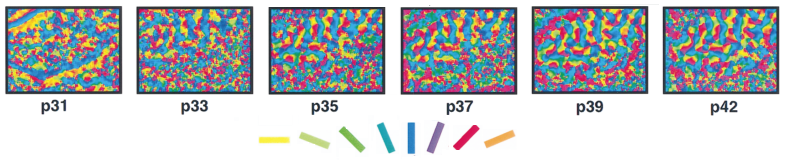
\includegraphics[width=0.9\textwidth]{Figure6.png}
	\caption[Development of an orientation map in ferret V1. Adapted
      from \cite{Chapman1996}.]{Development of orientation map in
      ferret primary visual cortex from post-natal day 31 to 42
      revealed using chronic optical imaging of intrinsic
      signals. Adapted from \cite{Chapman1996}.}
	\label{RFMapDevelopment}
\end{figure}

In the initial stages of development various preprogrammed guidance
cues set up the basic connectivity between the LGN and the cortical
processing areas \citep{Huberman2008}. Some successful models of
development have focused on the afferent connections between the LGN
ON and OFF cells and their targets in the visual cortex as the driving
force behind the development of orientation columns
\citep{Jin2011}. This is likely to tell only part of the story as even
during pre-natal development, retinal waves, consisting of periodic
activity in retinal ganglion cells (RGCs), spread across the retina
driving neighboring RGCs to fire in a correlated fashion, which allows
the primary visual cortex to develop topographic feature maps
\citep{Firth2005}. The most prominent proposals in theory and in
models have been focused on the termination pattern of both the
geniculocortical afferents in layer 4 \citep{Katz2000,Ringach2007} and
adjustments in feedforward and lateral connectivity through activity
dependent, competitive processes \citep{Bednar2003}.

It is now generally accepted that the development of topographic maps
is driven by activity dependent weight modification in some form of
Hebbian learning \citep{Shatz1996} and a variety of models have
emerged to account for this idea \citep{Bienenstock1982,
  Miller1989}. The LISSOM and GCAL models \citep{Bednar2003,
  Stevens2013}, which provide the basis of the modeling work proposed
in this project, have shown that robust map development can be
achieved with a small number of relatively simple mechanisms including
homeostatic plasticity, lateral gain control in LGN and lateral
connectivity in V1 \citep{Stevens2013} and will be considered in more
detail at a later stage. These models can account for the development
of orientation preference maps through both intrinsic activity such as
retinal waves \citep{Bednar2003} and visually induced retinal
activity. Experiments show that at the very least activity dependent
synaptic modification is required to achieve the finely tuned
precision, which can now be observed at single cell resolution
\citep{Ohki2005,White2007}.

Lateral intra-areal connections in particular have been implicated in
map development as their functional connectivity seems to be closely
related to map structure \citep{Gilbert1983}. Experiments in layer 2/3
of the tree shrew involving orientation preference mapping and
subsequent axonal staining have shown that although short range
connections show no preference in their terminations, long range
connections longer than 500 \si{\micro\metre} preferentially link
neurons with co-oriented and co-axially aligned receptive fields
\citep{Bosking1997}. In iso-orientation regions, cells therefore make
short-range connections largely with cells that prefer the same
direction as them, while at pinwheels short-range connections are made
with cells with a wider range of orientation preferences
\citep{Yousef2001}. However, it is known that the patchy lateral
connectivity in V1 does not arise until after the orientation map has
emerged \citep{Ruthazer1996}, indicating that they may be involved in
some higher-order processing not required during initial development.

The development of the early visual pathway is probably driven by a
number of mechanisms complementing each other at various stages,
starting with guidance cues setting up coarse predetermined
connectivity patterns, which are then refined through Hebbian
processes driven by internal and extrinsically stimulated
activity. Although the structure of a neuron's receptive field is
constantly changing and varies widely from cell to cell, a lot of work
has gone into measuring the exact structure and functional properties
of neural receptive fields and their underlying anatomical basis,
the neurite arbors.

\subsection{Functional and Anatomical Properties of Neural Receptive Fields}

The spatial properties of RFs in the LGN and V1 are of particular
interest in the context of this thesis as they provide the basis of a
realistic model of the para-foveal regions of the primary visual
cortex in macaques, allowing direct comparisons between model in
experiment in a system where the spatial scales are of great
importance. Before attempting to model the recurrent, lateral inputs
to V1, the spatial properties of each set of afferent connections
entering V1 need to be thoroughly understood and incorporated into the
model.

The extents and structure of neural receptive fields are defined by
the axonal and dendritic arborization of afferent, horizontal and
feedback connections, whether that is in the LGN, the V1 or higher up
in the cortical architecture. While these extents can theoretically be
measured physically by tracing the neurites of a number of cells, this
has only systematically been possible for thalamocortical
neurons, as tracing studies along the retinogeniculate
pathway are generally infeasible. Therefore spatial properties of LGN
RFs have been estimated through stimulus-driven protocols. The
following sections will outline the methods employed in characterizing
geniculate RFs and detail the relative contribution of afferent,
lateral and feedback connections to para-foveal RFs in the LGN and V1
of macaques.

\subsubsection{Receptive Fields in the Lateral Geniculate Nucleus}
\label{sec:LGNRF}

The spatio-temporal structure of receptive fields becomes increasingly
more complex when moving up in the visual processing hierarchy. As
described earlier, receptive fields in primate LGN are primarily made up
of antagonistic center-surround regions, although Gabor-like lobes are
also sometimes observed. Even at this early stage of processing,
lateral and feedback connections can modulate neural responses and
have been found to exert a suppressive effect \citep{Hubel1961}. More
recent studies have concluded that this suppressive effect is mediated
primarily by lateral connections and acts as a form of contrast-gain
control allowing for the encoding of a high dynamic range of luminance
values \citep{Bonin2005}.

As pointed out previously, the LGN receives a
large proportion of its inputs from feedback cells originating in
layer 6 of V1 \citep{Sherman2002}. It is unclear how these feedback
connections contribute to the RF properties of LGN neurons, but most
evidence suggests they are mainly involved in higher level modulatory
processes, especially in regard to the processing of motion
\citep{Sillito2006}, and thus do not directly contribute to the RF
structure.

Estimating the relative contribution and effect of the various LGN
afferents on its neural receptive fields has been attempted using a
variety of protocols. Unfortunately little to no data is available
from tracing studies, primarily because the LGN is embedded deep in
the brain, which makes it incredibly difficult to trace individual neurites
from and to their origin. Therefore a number of protocols have been
developed by which the parameters of the center-surround fields could
be estimated. After measuring the response of cat retinal ganglion cells
(RGCs) to moving bar stimuli \citep{Rodieck1965a,Rodieck1965b},
\cite{Rodieck1965} found that by fitting a Difference of Gaussian
(DoG) model to the data it was possible to estimate the relative
strength and size of the central and surround portions of the
receptive field. It was not until later that systematic recordings of
this kind were carried out in the LGN of macaques, at which point the
moving bar stimuli were replaced with sine gratings of varying spatial
frequency.

As not all papers can be reviewed here, the data from three different
studies with protocols of increasing complexity will be
considered. \cite{Derrington1984} was the first of such studies,
attempting to characterize the spatial and temporal properties of
parvocellular LGN neurons in \emph{Macaca mulatta} by fitting DoG
models to the responses. The analysis and confidence intervals of this
first study were rather limited, so the first study whose results will be
reported here is \cite{Spear1994}, which also considered the effect
of aging on receptive field properties. They found that the receptive
field center radius only increased very weakly with eccentricity, that the
smallest RF center radii were confined to parvocellular neurons, and
that the RF surround was significantly smaller in parvocellular
layers.

The next detailed study of LGN neural RFs was carried out by
\cite{Levitt2001}, investigating the effects of visual deprivation on
their visual response properties. There was a tendency for
parvocellular neurons to exhibit greater spatial resolution and the
highest temporal resolution to be magnocellular. Finally, their
analysis extended to earlier data from different species of macaque,
which showed that there is some variation in the distribution of ON
and OFF cells between \emph{M. mulatta} and
\emph{M. fascularis}. Overall their results on spatial tuning match
those found by previous studies quite closely, which is unsurprising
as the measuring and fitting protocols were highly similar.

In an attempt to calculate the relative contributions of different
neural connections, determine differences between the K-, M- and
P-cellular pathways and measure contrast dependent tuning, a number of
more recent studies have introduced more complex measurement and
fitting protocols. In particular, these experiments for the first time
attempted to separate out the influence of the non-classical or
extra-classical surround (ECRF or nCRF), which is thought to be
mediated by lateral and feedback connections. Therefore, a new
measurement and fitting protocol, introduced by \cite{Sceniak1999} in
form of the integrated DoG (iDoG) model to describe spatial summation
in the visual cortex, was used. Instead of measuring the response to
varying spatial frequency, this protocol involves the presentation of
drifting sine grating disks with varying apertures at the neuron's
optimum spatial frequency. The rationale behind this new protocol was
that the optimal spatial frequency would maximally drive the CRF
excitatory center, while minimizing the influence of the CRF
surround. Therefore the resulting area-summation tuning curve would
represent only the response from the CRF excitatory center and the
ECRF surround. The spatial frequency response measurement
protocol was also modified by confining the drifting sine gratings to a
circular aperture, reducing influences from beyond the CRF. While
these assumptions do not necessarily hold for reasons that will be
discussed later, they provide a first systematic attempt at separating
the contributions from the CRF and ECRF.

\cite{Sceniak2006} were the first to study spatial RF properties of
thalamocortical afferents in macaques by measuring both spatial
frequency and area summation response functions and fitting the
results with DoG and iDoG models (respectively) to estimate the
spatial parameters of the probed neurons. These results represent the
best estimates so far of the spatial properties of LGN receptive
fields. The first thing to note is the clear discrepancy between the
estimates of CRF excitatory center radius estimates in this paper
compared to previous estimates. This difference may be explained by
the more homogeneous distribution of cells, as the sample population
was taken exclusively from layer 4. The older protocol also failed to
confine the drifting sine grating to a disk, which may have resulted
systematic underestimation of the excitatory component due to
long-range suppressive effects. While excitatory extents vary hugely
across the various studies, the suppressive surround estimates are
fairly consistent. Furthermore, the spatial extent of the excitatory
CRF centers was found to be contrast invariant, while both the ECRF
and CRF suppressive surround extents were found to increase at lower
contrast levels. In summary, looking back at all the studies
considered here, excitatory CRF extents are generally distributed
between 0.05-0.5$\degree$ in radius, while inhibitory CRF and
suppressive ECRF radii are distributed distributed anywhere between
0.6-1.5$\degree$, and the suppression index is quite high
(SI\textgreater0.8) for 80\% of cells.

While these results provide the best estimates that are currently
available, the protocols used rely on a number of flawed
assumptions. The DoG model fitted to the spatial frequency tuning
curve relies on the assumption that no other components are
contributing to the response. Although the limited size of the sine
grating disk drive should \emph{reduce} long-range influences on the
response, and the ECRF surround is frequency invariant over a broader
spectrum than the CRF, further contributing mechanisms cannot be
excluded and may therefore affect the estimates. Similarly, the iDoG
model fitted to area summation tuning curves may be affected by a
number of unaccounted mechanisms. The iDoG model (see
equation~\ref{iDoG}) actually corresponds to an even-luminance disk of
variable size, rather than the sine grating disks that were used by
\cite{Sceniak2006}. The decision to use technically incorrect stimuli
was made to minimize the influence of the inhibitory CRF surround,
which may itself still have some influence on the response.  While all
these limitations should be kept in mind, this study is still the best
attempt at controlling unaccounted contributions, and thus provides
the best data on the spatial properties of macaque LGN RFs until
specific anatomical estimates are made available.

\subsubsection{Receptive Fields in the Primary Visual Cortex}

The receptive field properties of neurons in V1, in contrast to LGN
neurons, have been characterized to a far greater extent, with a number
of studies publishing direct anatomical data on neurite arborization
in addition to studies involving stimulus protocols such as those
employed to characterize LGN RFs. A number of reviews have been
published in the past decade to classify different portions of the
receptive field and link them to their physiological substrate in the
form of feedforward (FF), lateral, and feedback (FB) connections. In
order to attain a proper understanding of the spatial distribution of
afferent neurites populations of V1 neurons are targeted by, this
section will summarize the results.

Recent analyses have established a more complex model for the
classification of the spatial properties of neural RFs in V1 than the
simpler classical and extra-classical RF structure utilized in earlier
work. The structure of a V1 receptive field has been visualized by
\cite{Angelucci2006a} and can be seen in Figure~\ref{RFstruct}. It can
be broken down into the minimum response field (mRF), the summation
response field (sRF), which itself is broken down into the
high-contrast and low-contrast summation RF (hsRF and lsRF), and the
far surround. In particular, a distinction has been made between the
near surround, which extends as far as the lsRF, and a suppressive far
surround that extends beyond the lsRF. The distinction between the
hsRF and lsRF has been introduced to account for the contrast
dependence of size tuning. Problematically, not all studies nor even
all the latest studies use this means of defining different portions
of the RF, which has led to discrepancies in how the sizes of
different RF areas have been reported. The following sections will
attempt to integrate the results from studies employing different
means of classifying RFs.

The studies reviewed in \cite{Angelucci2006a} suggest that
geniculocortical FF projections integrate signals in the hsRF, while
lateral connections underlie the lsRF and may thus account for the
contrast dependence of spatial summation as well as modulatory effects
in the near surround. Classification through measurement of spatial
dimensions and onset latencies suggest that inter-areal FB
connections are responsible for modulatory influences from the
far surround. The influence and spatial properties of each of these
projections will be detailed in the following sections.

\begin{figure}
	\centering
        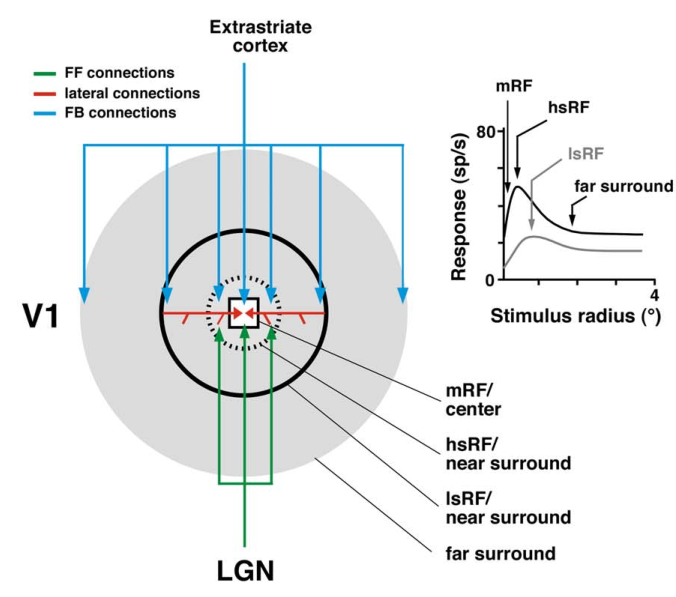
\includegraphics[width=1.0\textwidth]{angelucci_RFstruct.pdf}
	\caption[The structure of a receptive field in V1. Reproduced from
      \cite{Angelucci2006}.]{The receptive field structure of V1
      neurons showing the minimum receptive field (mRF), high contrast
      summation RF (hsRF) and low contrast summation RF
      (lsRF). Reproduced from \cite{Angelucci2006}.}
	\label{RFstruct}
\end{figure}

It is unclear whether this simple story attributing the different
parts of the receptive to specific projections is realistic, as there
will surely be overlap. Nonetheless, we will review the hypothesized contributions
to the receptive field in detail so we can later confirm whether the
different components in the model can actually account for the
contrast-dependent changes in receptive field integration.

\paragraph{Geniculocortical Afferents and the Minimum and High Contrast Summation RF} \label{AfferentBackground}

The primary visual cortex receives most of its driving inputs through
the three previously detailed M-, P-, and K-cellular geniculocortical
pathways. The M pathway principally terminates in layers 4C$\alpha$
and 6, the Parvocellular afferents terminate in layers 4A, 4$\beta$
and 6, while K cells primarily target layer 1 and some regions of
layer 3. By combining anatomical-tracing with physiological
recording the spatial extents of feedforward connections have been
measured in detail and linked back to the different RF regions.

The minimum response field as defined above is commensurate to the
classical RF and is usually mapped using drifting gratings masked to a
small disk of optimal parameters for that particular neuron. It is
surrounded by the high contrast summation RF, which is measured by
increasing the size of a drifting grating disk at high contrast until
the neuron reaches its peak response. Using a combination of tracing
and electrophysiological recording \citep{Angelucci2006a} found that
the visuotopic extent of LGN afferents matches the hsRF size of the
target V1 neuron. The diagram and bar chart in Figure \ref{FFmatch}
show how closely the estimates from tracing studies match the results
from physiological classifications of RF areas for magno- and
parvo-cellular pathways. The close match between these different
experiments suggests geniculocortical afferents may underlie the extent
of a V1 neuron's mRF. Recent evidence has also shown that the an LGN
neurons hsRF is roughly commensurate with a V1 cell's mRF. This seems
to suggest that the mRF of V1 cells is a product the summation of LGN
cells at their peak spatial summation, while the hsRF region of V1
neurons is defined by the integration of excitatory inputs from
partially suppressed LGN cells. Beyond that it seems likely FF
components partially contribute to surround suppression in V1, however
the spatial scales of surround modulation as well as its orientation
specificity seem to rule out LGN afferents as the major contributor to
the modulatory surround \citep{Angelucci2002,Angelucci2006a}.

\begin{figure}
	\centering
        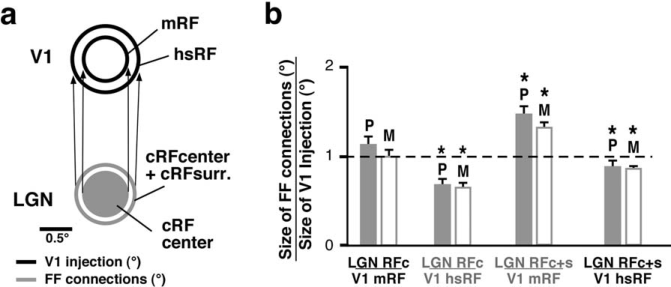
\includegraphics[width=1.0\textwidth]{angelucci_RFmatch.pdf}
	\caption[Comparison between anatomical and electrophysiological
      estimates of V1 receptive field extents. Reproduced from
      \cite{Angelucci2006}.]{Comparisons between electrophysiological
      characterization of RF structure and the spatial structure of
      geniculocortical projections to V1 in (a) diagrammatic and (b)
      chart form. Both demonstrate that the mRF and hsRF are
      coextensive with the spatial extents of geniculocortical
      afferents to V1. Reproduced from \cite{Angelucci2006}.}
	\label{FFmatch}
\end{figure}

Having established the contribution of geniculate afferents to the RF
of V1 neurons, it is time to look at their spatial distribution. In their
extensive studies and culminating review paper, \cite{Angelucci2006}
first fitted the iDoG to the spatial summation response curve of a
number of V1 neurons, then injected the recording sites with tracers and
measured the labeled connections and cell bodies. The linear
extents of the labeled connections were converted to visual field
coordinates using magnification factor (MF) estimates by
\cite{VanEssen1984}. The anatomical extent of the label was also
measured in the LGN and then converted to visual space coordinates using
MFs measured by \cite{Connolly1984} and LGN RF size estimates by
\cite{Derrington1984}. These calculations were used to arrive at the
aggregate receptive field (ARF) size, which takes the form:
%%
\begin{equation}
  ARF_{deg} = D^{\degree} + RF_{mean}
\end{equation}
%%
where $RF_{mean}$ is the mean RF size of cells recorded at the edge of
the injection site, which could reflect the mRF, hsRF or lsRF, and
$D^{\degree}$ is defined as:
%%
\begin{equation}
  D^{\degree} = D_{mm} / MF_{mm/deg} + S_{deg}
\end{equation}
%%
where $D_{mm}$ is the diameter, $MF_{mm/deg}$ is the magnification
factor and $S_{deg}$ is the RF scatter at the injection site. The
results show a close match between mRF and hsRF sizes as estimated in
V1 and sizes of the RF center and RF center + surround as measured in
LGN, once again reaffirming the idea that the mRF and hsRF are
primarily driven by geniculocortical afferents. The latest review
\citep{Angelucci2006} has measured the size of the hsRF in V1 neurons
of macaques at 2-8$\degree$ eccentricity as having mean of about
1$\degree \pm$ 0.1, which is roughly 2.2x larger than the mRF of the
same cell based on results from \cite{Angelucci2002} and
\cite{Levitt2002}. Estimates from the latest anatomical study
summarized in table \ref{electrophystable} are slightly higher,
with means of 1.09$\degree$ and 1.41$\degree$ in layer
4C$\alpha$ and 4A/C$\beta$ respectively.

In addition to the spatial extents of V1 RFs, \cite{Angelucci2006a}
also estimated the \emph{number} of LGN afferents that would contact an
individual V1 neuron. According to their estimates a single neuron in
layer 4C$\alpha$ can be expected to receive roughly 11 projections
from LGN M-cells. Although they were not able to put their own
estimates to the Parvocellular pathway, based on anatomical data from
cats they determined that on average 10 geniculate cells converge on a
V1 layer 4 cell, having observed only a maximum of ~30. They conclude
that the geniculocortical pathway in macaques exhibits an even lower
level of convergence than in cats.

\paragraph{Lateral Connections and the Low Contrast Summation RF}

% jbednar: why 'however'?  You haven't said they were exc->exc yet.
The patchy horizontal connections in the early visual cortex are one
of the most striking features in the cortex and have been proposed as
the mechanism for a number of observed phenomena, including the
contrast dependence of size tuning, which is why it is thought they
underlie the extent of the lsRF. Classically, however, developmental
models have assumed that lateral connectivity manifests itself through
short-range excitatory and longer range inhibitory connections
\citep{VonderMalsburg1973,Obermayer1990b}. The most striking property
of these connections is that they seem to link iso-orientation domains
as can be seen in Figure~\ref{BoskingLatExc}, which has implicated
them in a wide range of effects including long-range integration under
low-contrast conditions.

\begin{figure}
	\centering
        \includegraphics[width=0.6\textwidth]{BoskingLaterals.pdf}
	\caption[Patchy lateral connections overlaid on an orientation
      map. Reproduced from \cite{Bosking1997}.]{Illustrative
      examples of patchy lateral connections in the treeshrew visual
      cortex overlaid on an orientation map, clearly showing linking
      between iso-orientation domains. Reproduced from
      \cite{Bosking1997}.}
	\label{BoskingLatExc}
\end{figure}

The spatial scale of these connections has led several studies to
conclude that they may mediate modulation of RF-center properties in
the near surround \citep{Angelucci2002}. Lateral connections could
therefore provide a simultaneous mechanism for a number of observed
effects, including the expansion of the summation RF at low stimulus
contrast \citep{Sceniak1999}, co-linear facilitation
\citep{Mizobe2001}, and suppression from the near surround
outside the hsRF but within the lsRF
\citep{Sceniak2001,Levitt2002}. The previous section showed that such
phenomena could not be adequately accounted for by geniculocortical
afferents; measurement of spatial extents and response latencies of
horizontal connections reaffirm this view and have shown that the lsRF
and lateral connections are coextensive \citep{Angelucci2002}.

Apart from the exact spatial dimensions of horizontal connections, it
is important to highlight several other functionally important
properties. While layer 2/3 neurons display patchy connectivity,
linking regions with similar functional properties such as orientation
preference, this has been shown not to be the case in macaque layer 4B
and upper 4C$\alpha$ \citep{Angelucci2002}. In addition, it was found
that horizontal connections in macaque V1 are isotropic in visual
space, unlike the anisotropy along the axis of preferred orientation
observed in tree shrews \citep{Bosking1997} and several other
species. This could also indicate that orientation-specific contour
completion in macaques is mediated by feedback connections. Long-range
horizontal connections have been shown to elicit only subthreshold
responses \citep{Hirsch1991} and are thus limited to a modulatory
influence. However, as surround modulation extends far beyond the
monosynaptic spread of lateral connections, it is unlikely they
account for modulation from the far surround. Polysynaptic chains of
lateral connections are also an unlikely substrate for the far
surround due to the slow conduction velocity of their axons, and their
modulatory rather than driving nature. \cite{Bair2003} also showed
that onset latencies of suppression from the far surround were almost
equal to the delays from the near surround. This makes it likely that
far-surround modulation is mediated primarily by inter-areal feedback
connections, which we will look at in detail at a later stage.

Having established that spatial profile of lateral connections is
commensurate to that of the lsRF and vice versa, the data from both
sources will be laid out and analyzed. Anatomical data suggests that
the spatial spread of lateral connections can be anywhere between 3-10
mm (on average 6-7 mm) in total diameter \citep{Angelucci2002}. Along
its principal axis, the visuotopic monosynaptic spread of V1
horizontal connections has a mean of $2.47\degree \pm
0.3\degree$. This falls well within the range of estimates for the
lsRF as published in a number of studies
\citep{Shushruth2009,Sceniak1999,Sceniak2001}, which were fit with the
same integrated DoG model and stimulus protocol as used in the
\cite{Sceniak2006} paper on the spatial properties of LGN neurons,
reviewed previously.

In summary, there seems to be some agreement that lateral connections
could underlie the extent of the lsRF and mediate a number of effects
in the near surround, including contrast-dependent size tuning,
co-linear facilitation and iso-orientation contrast suppression.  The
extents of horizontal connections range between 3-10 mm, which
averages to around 2.5$\degree$ in visual space.

\paragraph{Feedback from Higher Cortical Areas and the Far Surround}

As the previous two sections have shown, modulatory influences to V1
RFs extend well beyond the spatial spread of both geniculocortical
afferents and horizontal connections. This extended modulatory field
is known as the far surround and is thought to be mediated by feedback
from higher cortical areas. The far surround has generally been
characterized as suppressive, especially for iso-oriented gratings in
the center and far surround. More detailed analysis has shown that the
far surround can also exhibit response facilitation under some
stimulus conditions. This section will characterize the function,
termination patterns and spatial extents of feedback connections from
higher cortical areas to V1.

The notion of a hierarchical organization of cortical visual areas has
been around for quite some time and more recent analysis of
feedforward and feedback connections has affirmed this view. At the
bottom of this hierarchy is V1, sending partially segregated FF
projections to areas V2, V3, V4 and the middle temporal (MT) visual area,
which all send FB projections back to V1
\citep{Felleman1991}. Feedforward projections from V1 to V2 arise
mainly from layer 4B and to a lesser degree from layer 2/3 and
6. Feedback connections, on the other hand, arise from layers 2/3A and
5/6 and terminate in the same layers from which FF connections are
sent, which means the cells projecting up the hierarchy often overlap
with the termination regions of FB projections being sent back down
\citep{Angelucci2002}.

Just like lateral connections, FB connections do not drive their target
cells, exhibiting only modulatory influence on the RF center
\citep{Bullier2001a}. Inactivation of areas V2 and MT has been shown
to reduce the firing rate of V1 neurons to stimuli in their RF center
\citep{Hupe1998}, suggesting FB inputs are summed with FF inputs to
increase activity. The exact balance between excitation and inhibition
of FB connections is so far not very well explored in macaques but
evidence from rats suggest that they almost exclusively target
excitatory cells. However \cite{Angelucci2006} and \cite{Schwabe2006}
have proposed a configuration where FB connections in the far surround
target pyramidal neurons, which in turn send monosynaptic horizontal
connections to excitatory and inhibitory neurons in the RF center and
can thus mediate both suppressive and facilitatory effects depending
on stimulus properties.

Feedback connections have been thought to underlie a number of top-down
effects in V1, including attention \citep{Treue2003} and the reverse
hierarchy theory of visual learning \citep{Ahissar2004}, but more
recent studies have suggested they contribute directly to the response
of V1 neurons to simple visual patterns
\citep{Angelucci2002,Angelucci2003,Schwabe2006}. Notably
\cite{Schwabe2006} and \cite{Ichida2007} seem to have resolved the
conflicting evidence about the far surround's dual suppressive and
facilitatory role. Using both experimental and theoretical work they
found that while the far surround is suppressive under high contrast
conditions, the response of a neuron to a low contrast stimulus in the
RF center is facilitated by a small annular stimulus in the far
surround. This indicates that excitatory and inhibitory surround
mechanisms have similar extents and that the sign of their
contribution depends on changes in local excitation/inhibition balance
brought about by surround stimulation.

Feedback projections from higher cortical areas to V1 mediate a number
of important contextual effects and have been implicated in the early
stages of visual attention, but also seem to be closely involved in the
processing of simple visual stimuli. This section has summarized
current knowledge on the spatial termination patterns of FB
connections to V1, indicating how they could give rise to functional
properties of V1 information processing. While the role of feedback
connections always needs to be taken into consideration, it will not be the
focus of this thesis, which will limit itself to afferent and lateral
connectivity in the primary visual cortex.  This limitation is
primarily for practical reasons, in that until suitable models of
extrastriate cortex are available, providing suitable feedback to V1
will remain very difficult and poorly constrained.

\section{The Internal Circuitry of Striate Cortex}

The previous section outlined the overall structure of the early visual
system, breaking down the contribution of inputs from various sources
on the receptive field (RF) of neurons in primary visual cortex
(V1). While this review provides general anatomical constraints and sheds
some light on the functional circuitry underlying many of the
contextual effects that have been observed in the primary visual
cortex, it does not address many of the fundamental questions about
the functional significance of recurrent cortical processing. In
particular, it does not address the delicate balance in both strength
and spatial extent between excitation and inhibition that is required
to halt runaway excitation, sparsify the inputs, and thereby allow for
the formation of concentrated activity bubbles around which
self-organization can take place. This section will cover how the
understanding of intra-cortical connectivity has evolved and how this
connectivity has been implemented in various developmental and
non-developmental models.

\subsection{The Mexican Hat} \label{MexicanHat}

Before complex tracing and circuit reconstruction techniques became
available, considerations about the connectivity profiles in the
cortex were largely theoretical or based on data from peripheral
regions, which were at the time more amenable to study. Anatomical
data and electrophysiological studies in the retina had shown that
there is a strong lateral inhibitory component involved in
decorrelating photoreceptor activities, thereby enabling more
efficient coding of the input \citep{Atick1992}. Lateral inhibition
was taken to be a general principle of sensory systems and, among
others, \cite{Blakemore1970} suggested repulsive interactions between
neighboring contours could account for psychophysical data. Further
evidence of lateral inhibition as a general feature of sensory systems
was provided by a variety of theoretical models of self-organization,
highlighting the necessity of effective local excitatory and 
long-range inhibitory interactions for the formation of local activity
bubbles, which in turn provided the basis for orderly map organization
\citep{VonderMalsburg1973,Miller1989}.

The connectivity profile employed in the various self-organizing map
models became known as the Mexican hat profile due to its strong
resemblance to a sombrero. A simulated Mexican hat profile is shown in
Figure~\ref{MexHat}, generated through a simple difference of Gaussian
(DoG) whereby a small excitatory Gaussian kernel is combined with a
larger inhibitory kernel. Numerous cortical models have successfully
employed this connection profile to explain a variety of effects
ranging from topographic map organization and orientation tuning to
contextual modulation. Problematically, it is unclear how biologically
realistic the assumption of strong local excitation and broadly tuned
and longer range inhibition really is.

\begin{figure}
	\centering 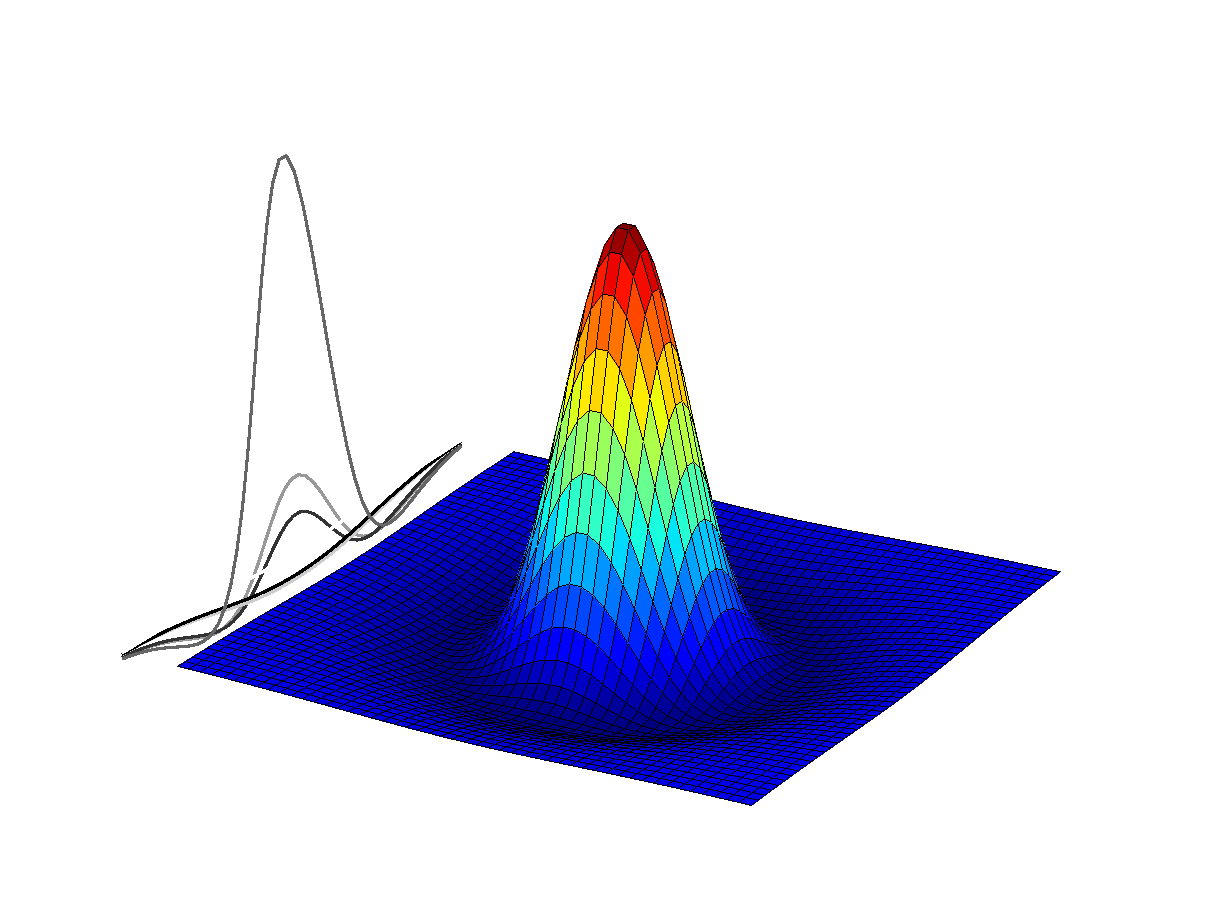
\includegraphics[width=0.7\textwidth]{mexhat.pdf}
	\caption{A 3D plot of stereotypical Mexican Hat connectivity.}
	\label{MexHat}
\end{figure}

The fundamental question then is whether there exists a set of
connections that could account for the local excitatory and
longer-range inhibitory component. A theoretical model by
\cite{Kang2003} suggests that a relatively small isotropic but fast
inhibitory projection could account for the inhibitory component of
the Mexican hat. To get a better understanding of how the Mexican hat
might arise from a circuit where the excitatory connections are
actually generally much longer, we will therefore investigate the specific
circuits involved.

\subsection{Contrast dependence of suppression}

An interesting but related phenomenon is that suppression and
facilitation can arise in the same neuron under under different
stimulus conditions. Specifically the contrast levels seems to have
complex effects on the overall sign of modulatory inputs to a neuron.

Electrophysiological and optical imaging have both confirmed that
strongly driven cortical neurons receive strong net local excitation and
long-range lateral inhibition \citep{Grinvald1994,Sceniak2001}. At
high contrasts \cite{Grinvald1994} showed that a neuron responding to
a small, central grating stimulus in isolation exhibits far greater
levels of activity than when presented with a co-linear surround
stimulus alongside the central stimulus. This highlights an
interaction between the center and surround RF that is not only
dependent on the orientation statistics but also on the contrast
levels in the input. In particular \cite{Hirsch1991} and
\cite{Weliky1995} showed that lateral connections impinging onto a
neuron would exert a small excitatory effect, when embedded in a low
contrast surround, while high contrast would flip the sign of these
contextual influences and suppress the central neuron's
activity. Additionally, \cite{Hirsch1991} found that laterally evoked
EPSPs, presumably underlying facilitatory effects, experienced strong
voltage-dependent enhancement, speculating that this effect would allow
stimuli in the surround to modulate cRF responses without driving the
response on its own.

Precisely how these two input-dependent modes of contextual
integration emerge is unclear. However, as anatomical tracing
techniques have become more sophisticated and biomarkers for different
cell types were discovered, attempts have been made at identifying the
different cell and connection types involved in this circuit. These
anatomical surveys showed that long-range connections extending beyond
a single orientation column were almost exclusively excitatory, and
80\% of these excitatory synapses target other excitatory pyramidal
neurons \citep{Hirsch1991,Kisvarday1997a}. The remainder of these
connections were shown to target inhibitory interneurons, which would
in turn contact pyramidal neurons, suggesting a di- or poly-synaptic
mechanism for long range suppression. On the basis of some of this
work \cite{Douglas1991} developed what has become known as the
canonical microcircuit for the neocortex. This circuit includes
separate inhibitory and excitatory neurons, which are driven by
thalamic afferents and recurrent connections. Further work has fleshed
out the spatial profiles of these connections, which ultimately gave
rise to the simplified circuit described in
Figure~\ref{V1MicroCircuit}. This proposal goes some way toward
reconciling anatomy with the experimentally measured functional
connectivity profile at high contrast levels.

\begin{figure}
	\centering
        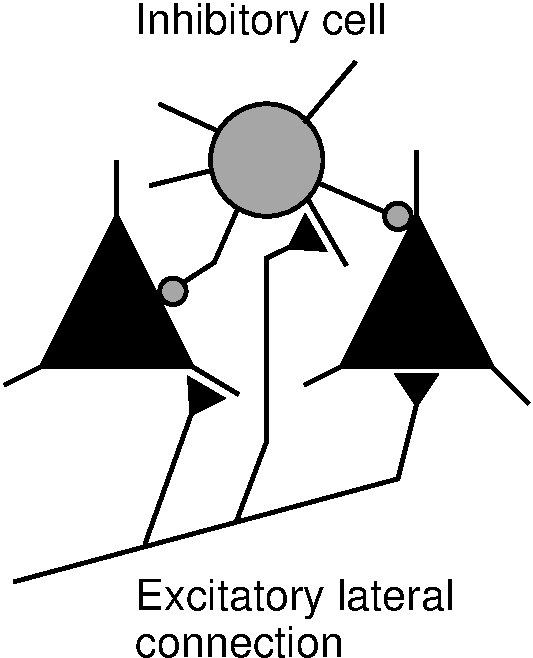
\includegraphics[width=0.25\textwidth]{weliky_microcircuit.pdf}
	\caption{Diagram presenting a proposed local microcircuit for
      long-range suppression through di- or poly-synaptic circuit in
      V1. Reproduced from \cite{Miikkulainen2005} as adapted from
      \cite{Weliky1995}.}
	\label{V1MicroCircuit}
\end{figure}

More recent attempts at reconciling anatomy with function have been
able to further resolve some aspects of the problem. In particular, there is
clear evidence showing that excitatory synapses onto excitatory and
inhibitory neurons differentially target their recipient
neurons. Excitatory connections onto inhibitory interneurons seem to
preferentially synapse perisomatically, in contrast with recurrent
long-range excitatory connections which have been shown to target
their recipient neurons dendritically
\citep{Gilbert1990,McGuire1991}. Additionally, at least a subset of
inhibitory interneurons seem to preferentially target the soma of
pyramidal and stellate cells they inhibit \citep{Markram2004}. On that
basis it is reasonable to assume that inhibitory connections are, in
general, stronger and may act divisively.

Although these divergent properties of excitatory and inhibitory
neurons were only discovered relatively recently, it had long been proposed that
inhibitory interneurons are inherently more effective at suppressing
activity than recurrent excitatory connections are at exciting the
network, but due to a high threshold or some other related mechanism
the inhibitory neurons are not strongly recruited unless there is
strong afferent input \citep{Sillito1979}, as would be the case under
high contrast conditions. Although it is now clear that network
effects allow for strong long-range inhibition through di- or
poly-synaptic connections under the right stimulus conditions, the
mechanisms by which contrast-dependent behaviors emerge from the
cortical circuit are still only vaguely characterized.

A number of models have been developed to explain contrast dependence
of contextual effects on the basis of the general principle of
asymmetry between the response properties of excitatory and inhibitory
neurons. One of the first to publish such a model were
\cite{Stemmler1995}, who suggested inhibitory neurons require higher
external input rates before activating because they receive
significantly less spontaneous background input as compared to
excitatory neurons, an effect known as stochastic resonance. Although
this mechanism has at least been theoretically reaffirmed
\citep{Bezrukov1997}, there is no experimental data establishing it as
a functionally significant mechanism in V1. Other models hoping to
account for a wider array of RF effects implement such a mechanism
directly by setting a higher threshold in the inhibitory population
and introducing very strong lateral excitation of inhibitory neurons
\citep{Schwabe2006}. Another suggestion was made by \cite{Somers1998},
who in addition to a simple threshold asymmetry, also point to the
claim by \cite{Thomson1994} and others \citep{Abbott1997,Tsodyks1997},
that synaptic depression causes recurrent excitation to quickly
decline in efficacy during high frequency stimulation, while
facilitation of excitatory synapses onto inhibitory interneurons
increases transmission efficacy as presynaptic firing rates increase
\citep{Thomson1995}.

The suggestion that inhibitory neurons have a higher contrast
threshold has become very popular in the theoretical literature of the
past 20 years. However, as of yet there is only limited evidence to
support this core assumption, and there are a number of alternative or
concurrent mechanisms that may explain all or at least some of the
contrast-dependent effects.

The fact that the V1 circuit seems to exhibit both a Mexican hat
profile and long-range facilitation, at least under some stimulus
conditions, seems contradictory. In particular, dissociating the
variety of different types of inhibitory interactions has been very
difficult from electrophysiological measurements alone. In order to
begin separating the origins of these different influences on a V1
neuron's response, we will therefore more closely investigate the
source of surround suppression in the cortex.

\subsection{Surround Suppression: Feedforward or Feedback?}

The last section highlighted how little we still know about the origin
of surround suppression and inhibition. There is still significant
controversy about whether surround suppression originates in feedforward or
feedback pathways or whether both contribute over different spatial
scales. The literature includes suggestions that suppression of the
classical RF by stimuli in the surround is mediated through synaptic depression in the
thalamo-cortical afferents \citep{Carandini2002}, broadly tuned
inhibition by thalamo-cortical recipients, long-range excitation of
local inhibitory interneurons, or even through various feedback
mechanisms. This section will detail the evidence for each of these
proposals and the possible anatomical origin of each of these mechanisms,
teasing apart the circuit by looking at interactions between
surround suppression, stimulus size, and contrast.

Since the circuitry of the cortex is so complex, the task of
identifying feedforward and feedback contributions to surround
suppression is difficult. Although only a starting point, one way of
roughly separating these two possible contributions is to look at
the time course of suppression. In the literature, early and late
contributors to surround suppression have been identified
\citep{Webb2005}. The early component is characterized as being driven
by lower CRF contrasts with spatio-temporally broadband tuning and
little adaptation \citep{Levitt1997,Cavanaugh2002a}. The late
component, on the other hand, is driven more strongly by high-contrast
stimuli in the CRF, has sharp spatio-temporal tuning, and can be
strongly affected by adaptation \citep{Levitt1997}. Evidence suggests
that the early, broadly tuned component originates in the LGN and the
thalamocortical recipient layer of visual cortex
\citep{Blasdel1984a,Hawken1996}. In monkey cortex in particular, this
broadly tuned suppressive effect is only weakly evident in the LGN and
is thought to arise much more strongly in layer 4 of striate cortex
\citep{Webb2005}, which may have some correspondence to the broadly
tuned inhibitory population identified by \cite{Hirsch2003}.

\cite{Carandini2002} on the other hand suggest that there is a
synaptic explanation for surround suppression, primarily due to the
speed with which the suppression arrives, its immunity to cortical
adaptation, and the fact that it is restricted to the CRF. However,
they concede that synaptic depression does not account for gain
control and the abolishment of cross-orientation suppression by
GABA$^{A}$ blockade, so a mechanism that can account for all these
phenomena may still be preferable. In that vein, \cite{Webb2005}
propose two inhibitory mechanisms, one of which sums local activity in
a neuron's CRF and divides the response of the CRF, and a later
component that receives inputs from a much larger area but provides
narrowly tuned suppression. The broadly tuned component in particular
has a strong relationship with contrast gain control, which has been
firmly established to act divisively. Independent work by
\cite{Xing2005} supports the suggestion of two inhibitory components
and further expands on the size dependence of these two
components. Specifically, \cite{Xing2005} conclude that the tuned component is
recruited far more strongly for larger stimuli, which seems to confirm
a contribution from beyond the CRF.

This recent work has identified two clear and distinct inhibitory
components, but has not yet fully described which mechanisms and
circuits by which they are mediated.  The next section will attempt to
address this shortcoming.

\subsection{Distinct Inhibitory Populations} \label{InhibitoryBackground}

In order to begin to understand the origin of intracortical surround
suppression mediated by various local inhibitory circuits, it is
necessary to consider the different candidate cell classes. While
there is a long list of different inhibitory cell types based on their
morphology and spiking behavior, recent techniques have divided
inhibitory cells into several broad, functionally distinct classes
based on their immunoreactivity. The two cell types considered here
are parvalbumin (Pv-ir) and somatostatin (Sst-ir) immunoreactive
neurons, which are primarily differentiated by the cellular locus of
their synaptic targets. While Pv-ir neurons seem to target pyramidal
cells perisomatically, Sst-ir neurons target their recipients
dendritically. Along with the Vasointestinal protein (VIP) expressing
interneurons these cell classes make up the majority of inhibitory
cells in the cortex. The following subsections will detail the
anatomical, physiological and functional differences between these
cell classes.

\subsubsection{Parvalbumin Immunoreactive cells}

The two main cell types that are immunoreactive to parvalbumin are the
chandelier and basket cells \citep{Binzegger2004}. While chandelier
cells make up only a small fraction of GABAergic neurons in the cortex
and are primarily found in layer 2/3, the fast-spiking (FS) basket
cells are the predominant interneuron subtype in the mammalian cortex
across all laminae, accounting for 42\% in layer 2/3 and layer 5 and
78\% in layer 4 of the cat \citep{Hogan1992,Huxlin2001} and up to 74\%
across cortical layers in macaque \citep{VanBrederode1990}. The
abundance in the thalamocortical-recipient layers and the fact that
they preferentially target the soma and proximal dendrites of spiny
neurons with multiple strong synapses, exhibiting high probability of
GABA release \citep{Freund2007,Markram2004}, ensures that basket cells
are of tremendous interest. On that basis it has been suggested that
the perisomatic connectivity profile of basket cells gives them the
ability to provide shunting inhibition to layer 4 spiny neurons,
acting divisively to control their response gain \citep{Wilson2012}.

Basket cells can be further subdivided, primarily based on their size,
into clutch and large basket cells. However, all basket cells can make
multiple connections onto a target pyramidal neuron
\citep{Somogyi1983} and have a considerable spatial extent
\citep{Kisvarday2002}. In particular, studies in cat area 17 and
macaque V1 have identified basket cells 1-2 mm in extent
\citep{Somogyi1983,Lund1987,Lund1991,Martin1983} and single-cell
tracing studies have even identified large basket cells, which give
off a roughly uniform number of boutons across a large diameter
extending up to two hypercolumns \citep{Buzas2001}, which corresponds
to about 1.5 mm in macaque. A schematic representation of the basket
cell connectivity profile is summarized and compared against both the
orientation column structure and the excitatory connection profile in
Figure~\ref{BasketCellExtent}. Functionally such a connectivity
profile may indicate that basket cells can suppress neurons with
widely varying orientations, which may implicate basket cells as an
important mechanism to sharpen orientation preference and would also
lead to cross-orientation contextual effects.

\begin{figure}
	\centering
        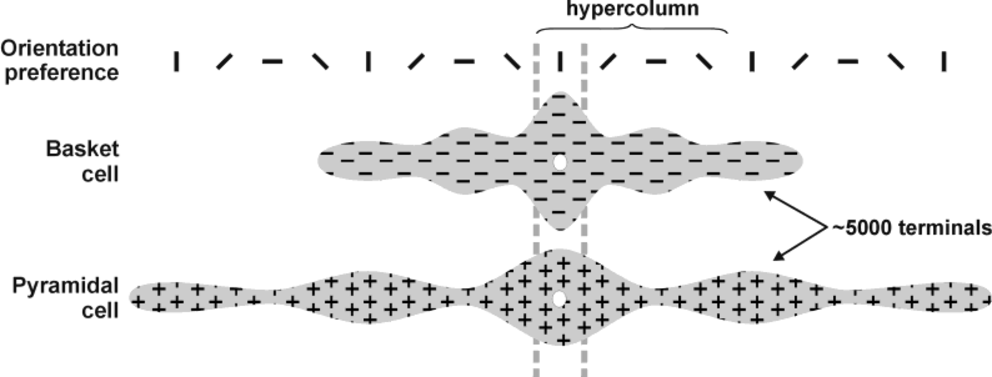
\includegraphics[width=1.0\textwidth]{basketcellextent.pdf}
	\caption[Schematic representing the proposed spatial distribution
      of pyramidal and basket cell extents and their relationship to
      the orientation map in V1. Reproduced from
      \cite{Buzas2001}.]{Summary schematic comparing relationship
      between long-range basket cell and excitatory connectivity with
      the underlying orientation preference structure. Upper legend
      represents different orientation domains in the cortical
      topographic map. Grey dotted lines indicate the orientation
      column within which the soma of the simplified basket cell and
      excitatory neuron are found. The grey field with minus signs
      indicates the extent of inhibition provided by the basket cell
      connections considered in the current study. The grey region
      with plus signs indicates the excitatory field of a
      stereotypical pyramidal cell, based on previous data by
      \cite{Bosking1997,Kisvarday1997a} and others. The height of the
      grey plus/minus regions indicates the number of axon terminals
      provided in that column. While basket cell terminals show local
      maxima every half hypercolumn distance, pyramidal cell terminals
      are maximal at every full hypercolumn distance. Reproduced from
      \cite{Buzas2001}.}
	\label{BasketCellExtent}
\end{figure}

In terms of their spiking behavior Pv-ir cells are typically
characterized as being fast fast-spiking (FS) neurons, often firing in
bursts with a very short response latency. It is important to note
however that not all fast-spiking cells are immunoreactive for
parvalbumin and that not all PV neurons are fast-spiking. Further,
evidence from somatosensory cortex in rodent and lagomorph species
suggests they receive strong input from thalamocortical afferents
arriving in layer 4 and very effectively suppress sustained firing
from spiny neurons receiving inputs from the thalamus
\citep{Swadlow2003}, implicating them in feedforward inhibition. A
possible feedforward inhibition circuit is shown in
Figure~\ref{burkhalterpv}. Their effectiveness in suppressing
feedforward activity can be explained by the large number of
thalamocortical axons they receive, which exhibit faster kinetics than
those targeting spiny neurons \citep{Cruikshank2007,Gabernet2005}, and
the fact that they evoke large inhibitory responses in spiny cells
\citep{Cruikshank2007,Gabernet2005}.

It is also important to note that the thalamocortical synapses onto
the Pv-ir population have been shown to be depressed by repetitive
activation, resulting in weaker feedforward inhibition at high
stimulation frequencies \citep{Gabernet2005}, a property which may
indicate lower activation of the PV population at high contrasts. The
Pv-ir population may also play an important role in network
homeostasis, as activity blockade has been shown to decrease the
efficacy of Pv-ir inhibition \citep{Bartley2008}, thereby indirectly
up-regulating activity in excitatory cells. Further, selectively
up-regulating Pv-ir cells using optogenetic stimulation was shown to
have a similar effect as lowering the contrast, which is to increase
preferred size and weakening surround suppression
\citep{Nienborg2013}. This evidence is compatible with the idea that Pv-ir
neurons provide strong feedforward inhibition such that the input
drive in the cortex is decreased, as would be observed under 
low-contrast conditions. Overall then, Pv-ir neurons show strong
interaction with stimulus contrast and may be involved in regulating
the gain of the network, with complex implications for the contrast
response of the network.

\begin{figure}
	\centering
        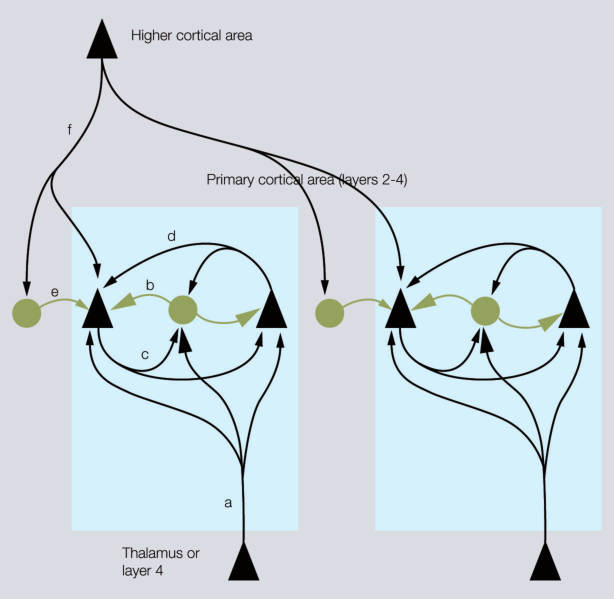
\includegraphics[width=1.0\textwidth]{burkhalter_pv.pdf}
	\caption[Proposed inhibitory circuit for feedforward inhibition
      mediated by PV cells. Reproduced from
      \cite{Burkhalter2008}.]{Inhibitory networks involving
      fast-spiking parvalbumin-immunoreactive neurons in
      thalamocortical, interlaminar, and interareal cortical
      circuits. Feedforward excitatory thalamocortical inputs to
      pyramidal cells, spiny stellate neurons ($\blacktriangle$) and
      fast spiking interneurons ($\newmoon$) in layers 2-4 (a). Inputs
      to interneurons are stronger (large arrowheads) than inputs to
      spiny cells. PV neurons provide strong (large rectangular
      endings) feedforward inhibition (b) to spiny cells. Feedback
      inhibition (c) results from PV neurons that are excited by the
      same spiny neurons that they inhibit. These reciprocally
      connected spiny neuron/PV neuron pairs share common inputs
      (e.g., cells in layer 4 from thalamus or cells in layer 2/3 from
      layer 4) creating recurrent excitatory (d) and inhibitory
      subnetworks (contained within blue shaded boxes). ‘Lateral’
      inhibition (e) of these subnetworks results from PV neurons that
      are driven by excitatory feedback connections (f) from outside
      the subnetworks (e.g., by layer 5 to layer 2/3 connections or
      feedback from higher cortical areas). Notice that ‘lateral’
      inhibition is weaker (small rectangular endings) than
      feedforward and feedback inhibition and impinges on multiple
      subnetworks. Reproduced from \cite{Burkhalter2008}.}
	\label{burkhalterpv}
\end{figure}

There is still considerable debate on the extent to which this
subpopulation is tuned to a particular orientation. Most
visuo-cortical models employ broad, non-specific GABAergic inhibition
\citep{Somers1998,Troyer1998}. This seems to be supported by
anatomical evidence, which has long shown that inhibitory projections
are generally diffuse and display low specificity for specific
stimulus features \citep{Albus1994,Kisvarday1997a}. Further,
electrophysiological data paints a similar picture, revealing
suppression that is broadly tuned for stimulus attributes, providing
orientation-unspecific suppression from a visual region that is
coextensive with the classical RF \citep{DeAngelis1992}. Recent
attempts at studying the Pv-ir neurons at the single-neuron level have
revealed a mixed picture. While the cells as a whole were broadly
tuned to various stimulus features, individual branches often
displayed very high specificity, which may underlie subfield
antagonism and contribute to a push-pull configuration
\citep{Kisvarday2002}. 

Studies in mouse visual cortex seem to confirm such a dual purpose of
Pv-ir neurons, although they also find higher heterogeneity in the
Pv-ir population \citep{Runyan2010}. This result may indicate a
laminar differentiation in function, as studies of Pv-ir neurons in
the thalamocortical recipient layer 4 have characterized them to
exhibit very broad tuning, due to their low spiking threshold and more
convergent inputs \citep{Ma2011}. However, even in layer 2/3 most
mouse Pv-ir cells displayed broad orientation tuning
\citep{Hofer2011}. Further studies in cat area 17 find very similar
results identifying a class of inhibitory complex cells in layer 4
exhibiting weak orientation tuning \citep{Hirsch2003}, which can
primarily be accounted for by the tuning of synaptic responses and a
lower spike threshold \citep{Nowak2008}.  A more recent study in
auditory cortex seems to affirm these conclusions, hypothesizing that
`while PV neurons may provide broadly tuned feedforward inhibition for
a rapid control of ascending inputs to excitatory neurons, the delayed
and more selective inhibition from SOM neurons may provide a specific
modulation of feedback inputs on their distal dendrites`
\citep{Li2014}. However, a more extensive study in layer 4 of the cat
found no significant broadening in the synaptic orientation tuning of
fast-spiking interneurons over that exhibited by regular spiking cells
in the same region \citep{Cardin2007}; only when looking at spiking
responses was a significant broadening found. As an explanation of
this apparent difference in tuning between rodents, which exhibit no
orientation maps, and primates or carnivorans, it has been suggested
that these cells pool the input from nearby neurons and inherit their
orientation preference \citep{Isaacson2011}. There may also be a
layer-specific segregation in their function providing push-pull
suppression in thalamocortical recipient layers and broader inhibition
in upper layers.

Based on our current knowledge of Pv-ir cell population and more
specifically the basket cells, it is clear that they provide a good
candidate mechanism to account for a number of important
phenomena. Their fast response profile, large spatial extent and
seemingly broader orientation tuning may allow them to carry out fast,
adaptive gain control and broadly tuned suppression, thereby
sharpening the orientation preference of the PNs in their vicinity.

\subsubsection{Somatostatin Immunoreactive cells}

The Sst-ir population has been characterized to a lesser extent, but a
general consensus is beginning to emerge around their function and
electrophysiological properties. The Sst-ir cells account for around
half of the non-PV-expressing neurons \citep{Gonchar2007,Xu2010} and
preferentially synapse onto distal dendrites and dendritic tufts of
pyramidal neurons \citep{DiCristo2004,Silberberg2007}, on the basis of
which it has been suggested that Sst-ir neurons act subtractively
\citep{Wilson2012}.

In trying to characterize the excitatory inputs to Sst-ir cells in
layer 2/3 of the mouse, \cite{Xu2009} determined that unlike Pv-irs,
the main source of excitation of Sst-irs were horizontal axons within
layer 2/3, not the ascending layer 4 axons. This property also
contributed to the size-dependent responses of the Sst-irs, which were
shown to be recruited progressively more strongly when they were
exposed to optogenetic photostimulation of increasing
diameter. Importantly, the Sst-ir response grew larger even when
photostimulation reached beyond its maximal dendritic extent,
demonstrating that the recruitment of increasingly more distant
pyramidal cells provided their main excitatory drive. This putative
circuit is shown in Figure \ref{som}, exhibiting their pooling of
tuned, excitatory input from pyramidal cells across a large area
yet providing only very local inhibition. It also seems that
Sst-ir interneurons are capable of disinhibiting the thalamocortical
recipient layer 4 by targeting Pv-ir cells \citep{Xu2013}.

In terms of their response properties, mouse visual cortex Sst-ir
neurons have been shown to exhibit much lower levels of spontaneous
and evoked activity, stronger orientation and direction selectivity,
and longer response latencies than Pv-ir neurons \citep{Ma2011}. These
properties are consistent across both layer 2/3 and 4 and may point to
a role in gating later-arriving intracortical excitatory inputs. In
terms of their tuning properties, Sst-ir neurons display smaller
On/Off subfields with less overlap than nearby spiny neurons and
orientation tuning, on par with pyramidal neurons. While most data on
their tuning properties comes from rodent visual cortex, which does
not exhibit a topographic organization of orientation tuning, it seems
the stronger orientation selectivity of Sst-ir cells can be accounted
for by their preferential connectivity to neurons with similar
orientation preference as well as a higher spiking threshold and
weaker excitatory inputs \citep{Bartley2008}. Another interesting
feature of Sst-ir response properties is the fact that although their
excitatory inputs are weak, those inputs are facilitatory, resulting
in delayed but strong activation under high frequency stimulation
\citep{Beierlein2003,Bartley2008,Tan2008}. Based on these properties,
Sst-ir neurons would only be recruited to provide significant
inhibition if the stimulus contrast or size reaches a certain level
\citep{Adesnik2012}. Thus they could provide a direct mechanism for
contrast-dependent size tuning and surround-modulation effects, being
only weakly recruited when contrast or stimulus size is low but
becoming strongly activated at higher contrast levels and for larger
stimulus sizes, providing a possible circuit mechanism for
\cite{Sillito1979} proposal for surround suppression.

Another suggested role for Sst-ir neurons is the gating of feedback
signals on the distal dendrites of principal neurons. Martinotti
cells, which provide strong axonal projections to layer 1 of the
cortex, make up a large proportion of Sst-ir neurons in layer 2/3 of
the cortex and are therefore well placed to suppress feedback signals
arriving in the superficial layers of the cortex
\citep{Fanselow2008,Gentet2012}. In the rodent somatosensory cortex,
\cite{Gentet2012} showed that Sst-irs in layer 2/3 become
spontaneously active during passive wakefulness but are strongly
suppressed during active whisking behavior, presumably by the
vasoactive intestinal peptide (Vip)-ir population discussed below. The
Sst-ir cells may therefore be involved in mediating top-down control
of sensory processing, effectively gating context-dependent processing
in a state-dependent manner.

\begin{figure}
	\centering
        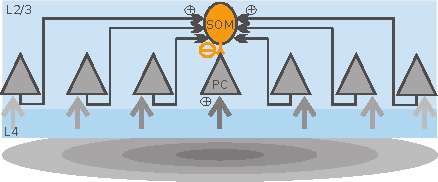
\includegraphics[width=1.0\textwidth]{adesnik_som.pdf}
	\caption[Schematic proposing Sst neurons' role in integrating
      long-range inputs. Reproduced from
      \cite{Adesnik2012}.]{Schematic illustration of the cortical
      circuit in layer 2/3 contributing to surround suppression. As a
      visual stimulus expands (larger stimuli are shown in lighter
      grey), recruitment of adjacent principal cells (PCs) increases
      Sst-ir excitation through horizontal axons (horizontal
      arrows). Reproduced from \cite{Adesnik2012}.}
	\label{som}
\end{figure}

In summary, Sst-ir neurons seem to provide delayed and
feature-selective feedback inhibition, which puts them in a good
position to effectively gate late-arriving intracortical excitatory
inputs originating in either lateral or feedback connections, but may
also be implicated in suppressing feedforward inhibition by
inactivating layer 4 Pv-ir cells.

\subsubsection{Vasointestinal peptide expressing interneurons}

The material reviewed so far has focused primarily on the two most
common types of inhibitory interneurons, the Parvalbumin (PV) and
Somatostatin-expressing (Sst) cells.  Since that initial work, a
number of studies have focused on the role of 5HT3ar-expressing
interneurons and particularly the vasointestinal peptide
(Vip)-expressing subgroup \citep{Lee2013, Fu2014, Higley2014,
  Kepecs2014}.

The Vip subgroup is particularly concentrated in upper, associative
layers and feedback layers of the cortex, as shown in
Figure~\ref{GABADistribution} by \cite{Rudy2011}. The most striking
finding was their central role in state-dependent modulation during
active whisking tasks in rodents. \cite{Lee2013} found that
S1-projecting vM1 pyramidal neurons strongly recruited Vip-expressing
interneurons in superficial layers of somatosensory barrel cortex,
which in turn inhibited somatostatin-expressing interneurons causing
effective disinhibition of cortical pyramidal cells. These results
were then affirmed through optogenetic stimulation of Vip neurons in
mouse V1, artificially mimicking the effects of locomotion
\citep{Fu2014}. When considered in conjunction with previous studies
that established strong cholinergic and nicotinic inputs to Vip
neurons from the basal forebrain \citep{Wickersham2009}, the evidence
suggests a strong involvement of Vip neurons in a cortical circuit
responsible for the enhancement of activity in sensory cortex by
behavioral state.

\begin{figure}
	\centering
        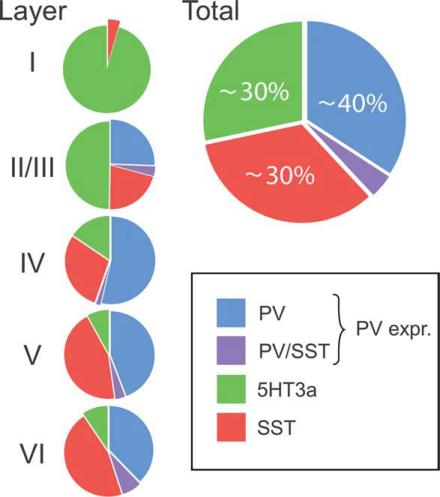
\includegraphics[width=0.4\textwidth]{GABADistribution.pdf}
	\caption{Distribution of GABAergic interneurons in mouse S1 cortex
      by immunohistological marker. Reproduced from \cite{Rudy2011}.}
	\label{GABADistribution}
\end{figure}

\subsubsection{Connectivity between different cell types}

In order to gain an understanding of the circuits the different
interneuron cell types are involved in, it is important to consider
their interconnectivity. Several studies have sought to determine the
connectivity between Pv-ir, Sst-ir and other interneuron types. The
core findings of these studies determined that Pv-ir cells
preferentially inhibit one another, Sst-expressing cells avoid one
another and inhibit all other types of interneurons, particularly the
Pv-ir cells \citep{Xu2013}, while a third type, the Vip-ir cells
preferentially inhibit Sst-ir cells \citep{Pfeffer2013}. This
connectivity profile is schematically represented in
Figure~\ref{gaba_circuit}. In mouse cortex the Pv-ir, Sst-ir and
Vip-ir cells accounted for about 40\%, 18\% and 8\% of the GABAergic
population, respectively \citep{Xu2010}, and although these
percentages vary considerably across species Pv-ir and Sst-ir are
always the two most commonly expressed GABAergic populations.

\begin{figure}
	\centering
        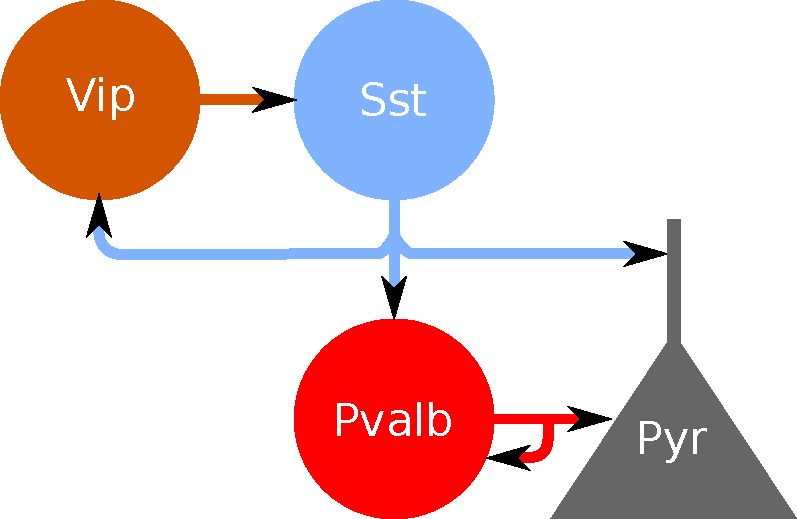
\includegraphics[width=0.7\textwidth]{pfeffer_gabacircuit.pdf}
	\caption{Connectivity between somatostatin (Sst),
        parvalbumin (Pv), vasoactive intestinal peptide (Vip)
        expressing and pyramidal (Pyr) cell types. Adapted from
        \cite{Pfeffer2013}.}
	\label{gaba_circuit}
\end{figure}

\section{GABAergic regulation of plasticity and column structure}

Experience-dependent plasticity has been shown to shape the
organization of the sensory cortex during an initial critical period and
beyond. Dark-rearing \citep{Fregnac1978} and monocular-deprivation
(MD) experiments \citep{Shatz1978} in particular have confirmed the
fundamental importance of sensory experience in shaping the
development of the cortex. The mechanisms controlling the onset of the
critical period and regulation of plasticity thereafter have also been
studied extensively.  A large body of evidence points to the
important role of the inhibitory neurotransmitter
$\gamma$-aminobutyric acid (GABA) in regulating synaptic
plasticity. However, as the above paragraphs have shown, the population
of GABAergic neurons is highly heterogeneous with hugely divergent
anatomical and functional profiles. Using specific pharmacological and
genetic populations, it has been possible to narrow down the
involvement of certain interneuron subtypes in shaping critical-period
plasticity and column structure in the cortex.

One of the first indications that GABAergic circuits are involved in
shaping plasticity came when it was shown that a gene-targeted
disruption of the GABA synthetic enzyme glutamic acid decarboxylase 65
(GAD65) could delay critical period onset indefinitely
\citep{Fagiolini2000}. In order to further narrow down the specific
GABA circuits underlying visual cortical plasticity, more specific
pharmacological manipulations were required. On that basis
\cite{Fagiolini2004} used benzodiazepine infusions, known to
selectively enhance GABA type A ($GABA_A$) receptor-mediated currents
through the $\alpha1$ subunit \citep{Rudolph1999}, in conjunction with
MD to prematurely trigger ocular dominance plasticity in mice. These
$GABA_A$ receptor-$\alpha1$ subunits are preferentially enriched at
somatic synapses receiving input from Pv-ir large basket cell
terminals \citep{Klausberger2002}, strongly implicating large basket
cells in visual cortical plasticity.

Beyond controlling the timing of critical period plasticity, further
experiments using benzodiazepines have shown strong effects on the
columnar organization of the cortex. The experiment by
\cite{Hensch2004} locally infused regions of cat area 17 with the
$GABA_A$ agonist diazepam and an inverse agonist (DMCM) and studied
the effects on ocular dominance columns. Chronic treatment with
diazepam had little effect in the functional properties of mature
cortical neurons in vivo apart from enhancing inhibitory postsynaptic
currents. However, the treated hemisphere exhibited reduced
binocularity of single unit responses and wider OD columns near the
infusion site. Infusion with the benzodiazepine inverse agonist DMCM
had the inverse effect, resulting in less discrete and narrower
columns near the infusion site. These results suggest that the
diazepam-mediated enhancement in competition reduces binocularity of
single-unit responses, as well as sharpening and widening the
anatomical segregation of monocular regions near the infusion
site. This once again suggests that $GABA_A$ inhibitory currents,
primarily originating from Pv-ir neurons in the cortex, are
fundamentally important to shaping the plasticity and organization of
the cortex.

In order to establish how ocular dominance plasticity emerges during
monocular deprivation, \cite{Kuhlman2013} developed even more
precisely targeted pharmacological manipulations. By selectively
expressing specific receptors on Pv-ir cells they were able to
selectively up- and down-regulate their activity. Their results
indicate that a rapid but transient reduction in Pv-ir cell firing
restores pyramidal cell firing to pre-deprivation levels, allowing
competitive plasticity to occur. Pv-ir neurons therefore seem to play
a permissive role in visual cortical plasticity. Interestingly, adult
sensory plasticity such as reinforced associative learning occurs
through a similar mechanism, where cholinergic activation of layer 1
interneurons suppresses Pv-ir neural activity allowing associative
fear learning to occur \citep{Letzkus2011}. All this work suggests a
crucial role for Pv-ir neurons in controlling cortical plasticity
during the critical period and beyond.

\section{Contextual Modulation and Attention} \label{contextualmodulation}

Arguably, the computational task in vision is to map visual experience
to the cortical representation of that particular stimulus or if no
such representation already exists, to extract lower level features in
order to encode them for future reference. Using this statistical
model the brain is then able to decide which visual features carry
behavioral importance and which can be safely ignored. As such the
neocortex has to combine prior information with the incoming
information stream and quickly and reliably identify the most salient
stimuli. It has often been argued that this process is mediated by
bottom-up and top-down processes, although it seems likely that there
is close coupling between the two. This section will outline
high-level models of attentional modulation, and attempts to
understand the neurobiological processes behind them and more basic
contextual modulation phenomena that may underlie many of these higher
level effects.

\subsection{Contextual and Attentional Phenomena in V1}

A number of phenomena associated with attention and contextual
modulation, including iso-orientation suppression or facilitation,
boundary detection, contour completion and noise exclusion have been
observed in V1. Although these phenomena are generally associated with
bottom-up attention, they lay the foundation for higher level phenomena
such as pop-out and figure-ground segregation and may reveal more
about general mechanisms applying also to higher visual areas.

Basic contextual effects such as iso-orientation suppression have
already been discussed and models have begun to suggest the functional
connectivity mediating implicating both lateral and feedback
connections. \cite{Li2002} has proposed that pre-attentive
bottom-up processes allow V1 to generate a saliency map of the visual
input. However, the fact that higher cortical areas have also been
associated with saliency signaling and the lack of long-range
intra-areal connectivity in V1 suggest that while it can encode local
saliency, feedback is required to globally integrate saliency across
visual space.

Feedback modulation of V1 activity has been implicated in a number of
effects, spatial attention being chief among them. Spatial attention
is thought to be able to select multiple low- and high-level objects in
the visual space across V1 and higher visual areas
\citep{McMains2004}. Spatial attention is thought to underlie noise
exclusion \citep{Dosher2000} and may be explained by effects similar
to what has been experimentally observed during iontophoretic application
of ACh. Other effects that have been commonly associated with
feedback in some form are the signaling of illusory contours, which
have been shown to be negatively signaled or deemphasized in V1
\citep{Ramsden2001} and boundary detection \citep{Poort2012}.

\section{Natural Image Statistics, Sparsity and Horizontal Connections}

It has long been hypothesized that connectivity in the cortex captures
the statistics of the sensory input in order to perform predictions
and maintain sparse representations of subsequent inputs \citep{Field1993,
  Simoncelli2001}. These effects cover both that the distribution of visual
features that are thought to sparsely represent the visual features of
world \citep{Olshausen1996}, but also suggests that it captures the
Gestalt law of good continuation in the form of so-called association
fields, which preferentially link neurons which represent edges on a
continuous contour \citep{Field1993}. Separately a wide range of work
has explored the distributions of light intensities, color statistics
and spatial correlations in natural images. In particular, the
power-law distribution of spatial frequencies in natural images has
been widely discussed in the literature, but ultimately this property
largely seems to reflect scale invariance within natural images
\citep{Ruderman1997}.

Numerous studies and models have since been devised to address whether
the visual system takes advantage of the correlational structure of
natural images. These types of normative models were able to show that
surround inhibition, whether subtractive or divisive, could cancel out
correlations, effectively whitening or decorrelating the activity in
the visual system \citep{Srinivasan1982, Atick1992}. In doing so they
quickly found that simple decorrelation was not sufficient to
optimally represent natural images, because whitening does not
eliminate all structure in a natural image; e.g., edges and lines
remain. By introducing an explicit sparsity constraint,
\cite{Olshausen1996} were able to develop V1-like simple cell
receptive fields with varying orientations, spatial frequencies and
sizes. These models suggested that the sensory system was optimizing
two constraints, sparsity and statistical independence. However, even
these approaches cannot achieve complete statistical independence,
since there are higher-order correlations even between non-overlapping
receptive fields.

By introducing divisive normalization, \cite{Schwartz2001a} were able
to show that these types of dependencies could be further
eliminated. Furthermore, the weights used in the computation of the
normalization signal could be specifically optimized to maximize the
independence of the normalized responses. Additionally, they
demonstrated that the optimal weights were at least partly due to the
prevalence of extended contours in natural images.

Attempting to quantify the co-occurence statistics of contours in
natural images, \cite{Geisler2001} demonstrated that the performance
in contour-detection tasks could be predicted by a local grouping rule
derived from the co-occurence statistics. The first explicit link to
horizontal connectivity was made by \cite{Sigman2001}, who noted that
the pattern of long-range patchy connectivity in the primary visual
cortex linking iso-orientation columns has a close correspondence with
the observation of co-circularity in natural image statistics. Noting
the processes of iso-orientation suppression and contour integration,
they argue that iso-orientation suppression may serve to further
reduce redundancies in neural coding, thereby achieving greater
statistical independence, which would explain why neural responses
appear most sparse when presented with natural stimuli. Furthermore
recent findings have shown that low-level co-occurrence are sufficient
to classify images of animals \citep{Perrinet2015}, suggesting that
even early visual areas could be involved in high-level classification
tasks. Secondly, observing that visual cortex can also exhibit
co-linear facilitation under low-contrast conditions
\citep{Sceniak1999, Kapadia1999}, they suggest that under low
signal-to-noise conditions the cortex may act to enhance commonly
encountered patterns to aid the identification of contours and form.

These theoretical studies have hugely advanced our thinking about the
computations performed by the early visual cortex, yet very little
work has been done to look at the actual structure of horizontal
connectivity in V1, largely due to the difficulty in obtaining data
from more than just a few cells. Even on the question of whether
horizontal connections are anisotropic along the axis of preferred
orientation of the neuron, as would be expected from theoretical
studies, there is conflicting evidence. The result has been confirmed
in monkey \citep{Sincich2001}, tree shrew \citep{Bosking1997} and cat
\citep{Schmidt1997}, but conflicting results have been reported for
macaque \citep{Angelucci2002}. By performing analyses on a tree-shrew
dataset from 1997, \cite{Hunt2011} investigated whether horizontal 
connections captured the co-circularity of natural image
statistics. Although they found neurons that exhibited co-circularity
and anti-cocircularity and hypothesize a role for both, given the
small number of lateral connections fields and the fact that
second-order properties are highly sensitive to even small errors in
the data, it is unclear how strong this result is. Further research in
this area is desperately needed if we are to understand how the
patterns of lateral connectivity relate to natural image statistics.

\section{Existing large-scale models of the primary visual cortex}

In the previous sections we laid out a wide range of evidence
relating specific empirical studies to each other, to begin teasing
apart how low-level interactions can give rise to complex behaviors. A
wide range of modeling work has been targeted to that very
question, and there exists a wide breadth of models attempting to model
the function of the visual cortex at the level of individually spiking
neurons or modeling looking specifically at the surround modulation
interactions between neurons. Here we will review some of these
models, highlighting why although many models explain specific
phenomena well, the lack of development and learning means that these
models are static and cannot easily explain the dynamic, adaptive
nature of computation in the cortex.

\subsubsection{Large-scale spiking models} \label{LargeModels}

With the introduction of increasing computational power it has become
feasible to model large networks of spiking neurons, allowing
simplified models of the visual cortex to be created. In particular,
large scale simulators such as NEURON \citep{Hines1994}, NEST
\citep{Gewaltig2007} and interfaces such as PyNN \citep{Davison2009}
have made it possible to specify complex neural network models at the
level of individual neurons and even synapses and ion channels.

These models generally replicate the statistics and rough spatial
scales of different types of connections, between different cell
classes and investigate the response of the model at resting state or
when provided with thalamic input \citep{Shelley2002,
  Potjans2014}. Additionally there are also even larger models
attempting to model the visual cortex just as one area of a complex
brain network \citep{Eliasmith2012}. What these models have in common
is that they are not well suited towards addressing the kinds of
question most vision scientists are interested in, particularly in
regard to the way the visual cortex can extract and encode the
statistics of the visual input and give rise to well-studied effects
like contextual modulation. Instead these models are usually used to
study only the overall statistics of the responses. As an example,
\cite{Potjans2014} develop a highly detailed and refined microcircuit
model of the visual cortex, including different cell types and laminar
distributions, which they can scale to large cortical networks. The
resultant model can provide answers about the flow of information in
the network between different layers, but because it is simply a
statistical model of connectivity it cannot address questions at the
functional, algorithmic, or computational levels.

Alternatively, there are large-scale models that disregard the
architecture of different brain regions entirely, instead treating
them as modules of excitatory and inhibitory cells serving
a specific function. \cite{Eliasmith2012} present one such model,
which models the entire cortical hierarchy and even performs specific
tasks. Here the model of V1 is simplified to the point where it is
simply a visual encoder, ignoring more complex interactions entirely.

As we have seen, models of this scale suffer of one of two
problems. When incorporating a lot of biological detail, they are very
useful for understanding the low-level interactions in a network and
how information is communicated locally, but are not usually useful
for linking low-level processes to the higher-level processes that
these processes underlie. Models at the other extreme are relegated to
be very high-level approximations of the visual cortex, without the
full breadth of complex contextual effects that has been observed in
the visual cortex.

\subsubsection{Surround modulation models} \label{SRmodels}

Perhaps the precisely opposite approach to building in copious amounts
of biophysical detail is to focus on a particular phenomenon and
attempt to explain it with a reduced set of mechanisms. These models
have traditionally been incredibly useful in explaining different
aspects of the literature in V1. Specifically, point, rate-based
neuron models have been used to explain effects ranging from surround
suppression and to more complex contextual-modulation effects such as
contour integration and pop-out.

The surround-modulation literature is one of the most complex topics
in visual neuroscience, due to the high dependence of the observed
phenomena not only on the precise stimulus conditions but also the
behavioral state of the animal. As we discovered in
Section~\ref{contextualmodulation}, there are two main phenomena that
are of interest: surround suppression, usually thought to reduce
redundancy in the input, and contextual enhancement of responses
through facilitatory effects. These two opposing mechanisms are
thought to drive a wide range of the phenomena in the literature
including pop-out, contour completion, as well as end stopping,
flanker facilitation, and much more.

Various models have been proposed to explain how these contextual
influences emerge. In one of the more straightforward models,
\cite{Li2002} proposes that through recurrent enhancement of
responses, long-range lateral connections can give rise to a visual
saliency map in V1, which underlies pop-out, enhancing features that
stand out from the visual background. While this model explains how a
particular surround modulation effect can emerge from the network
interactions between neurons with different tuning properties, it does
not account for both suppressive and facilitatory effects and since it
is highly abstract cannot shed light on the precise interactions that
could give rise to both in a circuit.

Other models such as the \cite{Schwabe2006} model break down the
interactions from different sources in more detail demonstrating how
long-range patchy horizontal connectivity can mediate both excitatory
and inhibitory influences from the surround. Unlike previous models
they suggest that long-range feedback connections could be the main
driver of these contextual influences and that the drive to inhibitory
neurons in the local circuit determines the sign of the
effect. However, since this is a static model it provides no account
of how the required lateral or feedback connectivity could emerge and
since the model only represents 1D space cannot process realistic
stimuli. Additionally this model still uses the assumption originally
made by \cite{Somers1998}, that inhibitory neurons have a higher
threshold than excitatory neurons, to account for contrast dependent
effects, which has received little experimental confirmation.

An alternative to this circuit-level analysis is to express these
interactions in the more abstract framework of predictive coding. The
work by \cite{Spratling2010} in particular expresses the cortical
circuit as predictive coding, modeling the response of V1 neurons
using a competitive mechanism between neurons attempting to best
represent the input. Like many others, this model provides a good
account of various surround modulation effects including iso- and
cross-orientation suppression but exhibits only weak facilitatory
effects, suggesting that it does not fully capture the mechanism that
is behind the contrast- and context-dependent interactions between
suppression and facilitation. Furthermore, it is very difficult to
relate the interactions between explicitly predictive or error-coding
neurons to the real interactions taking place in the cortex.

Then there are a class of phenomenological models attempting to
explain a variety of surround modulation effects based on the
geometries found in visual fields and the Gestalt law of good
continuation \citep{Field1993}. The \cite{Keemink2015} model, for
example, suggests that effects including the tilt illusion and contour
detection can be explained by a single mechanism, which computes the
elastica curvature energy of the smoothest contour connecting oriented
bars. This suggests that the visual cortex can somehow compute the
energy required to connect different contours but does not explain how
this association field could emerge. It is therefore a good account of
what the cortex is computing, but does not provide a canonical
mechanism for how these interactions can emerge independent of the
sensory modality that is involved. A general mechanism would allow the
model to extract the statistical dependencies between arbitrary
features, such that when trained on natural images it automatically
extracts the geometric relationships within contours.

Another avenue of study has been the approach by the Schwartz lab, who
have for a long time investigated the interaction between
natural-image statistics and surround-modulation effects. This is
perhaps one of the most interesting approaches, because it treats
contextual phenomena not as a by-product of some underlying
computational process, but rather supposes that they are driven by the
statistics of the visual input and are therefore closely tied to the
computational task that is actually being solved. In \cite{Coen2015}
they describe an extension of a simple normalization framework that
computes the homogeneity in an image between center and surround,
gating the divisive normalization component accordingly, which
directly leads to feature-specific surround modulation effects
observed in experiments. In this framework, surround modulation is
simply the measurable effect of statistical inference, improving the
efficient encoding of the stimulus.

All of these models capture important parts of the phenomena involved,
highlighting how network interactions between neurons with different
tuning properties can give rise to complex contextual modulation
effects \citep{Li2002}, where the sources of this input could
originate from \citep{Schwabe2006} and how these interactions might
fit into a general computational paradigm that is concerned with
prediction and inference \citep{Spratling2010, Coen2015}. However, all
of these models are static, presupposing an existing profile of
connectivity, and thus cannot directly address how different cell
types could interact to give rise to a circuit, mechanistically
explaining how these effects emerge.

\subsection{Developmental models} \label{devmodels}

As it is thought that the cortex captures statistics about the sensory
streams to construct internal models of the world, it is clear that
function, structure and development are closely linked. Indeed it is
now clear that V1 is a dynamic and adaptive circuit, which exhibits
learning and learns to optimally encode and represent its inputs. In
other words, V1 is not a static circuit, organizing solely based on
genetic cues, but rather self-organizes through a complex interplay of
genetic triggers, intrinsic mechanisms such as retinal waves and
perhaps most importantly, external visual input. A number of models
have been developed using these ideas, explaining the development and
self-organization of the V1 circuit as fundamentally being driven by
activity-dependent and correlation-based processes.

The original principles for what became the class of self-organizing
map (SOM) models were first formulated by \citep{VonderMalsburg1973},
who recognized this connection and sought to explain the
self-organization of neurons into topographic maps via the simple
process of Hebbian learning. The \cite{VonderMalsburg1973} model
showed for the first time that very simple mechanisms such as Mexican
Hat (Section~\ref{MexicanHat}) connectivity can give rise to the
smooth organization of individual neurons into a topographic map.

Since then many models have sought to explain the
self-organization of individual neurons into an overall functional
circuit, which can extract and encode a wide range of features in
sensory input. The paradigm has been applied not just to visual
neuroscience but also the auditory, somatosensory, and olfactory
cortices. There now exists a wide range of literature arguing to what
degree the self-organizing processes are driven by the afferent,
excitatory and inhibitory components. In particular the development of
orientation-selective simple and complex cells has received
significant attention.

Applying this correlation-based paradigm, \cite{Miller1989} were able
to show that the development of realistic stripy ocular dominance
columns could be explained, demonstrating the role of neurons
competing to represent specific visual features in the input. The
\cite{Somers1995} model also applied this paradigm, once again to the
development of orientation selectivity.  They argued for a strong role
for recurrent excitations to bind the responses of neurons together,
which strengthens the weak orientation selective input from the
thalamus, with strong unselective inhibition keeping the circuit in
balance and sharpening the orientation tuning of the principal
neurons.

The idea that the development of highly complex cortical circuits can
be explained using a small set of mechanisms therefore has received a
significant amount of attention and has been able to explain the
development of not just visual receptive fields but also somatosensory
\citep{Wilson2010}, auditory \cite{Khan2011} and other feature
maps. The fundamental principles underlying these computations are
generally the same, with individual neurons competing to represent an
input, leading to a smooth mapping of an underlying feature of the
input onto the cortical surface. So while the precise process which
allows neurons to compete and the learning rule that allows these maps
to robustly, yet adaptively develop has not been conclusively
established, a lot is now known about self-organization of the cortex.

In recent years some effort has been put into making the SOM-based
models more closely represent the functional organization of the
cortex, starting with the LISSOM model \citep{Bednar2003} and more
recently the simpler and more robust GCAL \citep{Stevens2013}
model. In these models the retina, LGN, and V1 are modeled as a set of
neuronal sheets with feedforward and lateral connectivity
self-organizing into the complex topographic maps. These models
provide a very good match to the known developmental time course and
replicate a large range of phenomena observed in the mammalian cortex,
yet work with only a small set of mechanisms including contrast-gain
control, an adaptive per-neuron threshold, normalized Hebbian
learning, and lateral connectivity 
\citep{Stevens2013}. Extensions of this model explaining the
development of complex cells and of contrast-dependent size tuning
\citep{Antolik2011} as well as a continuous time model matching LGN/V1
temporal response functions have also been developed
\citep{Stevens2011}.

The GCAL (gain control, adaptive, lateral) model is based on several
core observations about information-processing in V1 and the cortex in
general. As previous sections have shown, the primary visual cortex of
primates responds strongly to specific low-level features in its
visual input, including orientation, color and direction. Selectivity
to these features is conserved across a wide range of contrasts, and
neurons form topographic feature maps across the surface of V1 by
virtue of self-organization.

While these experimentally confirmed findings are specific to vision,
the concept of equipotentiality proposes that different areas in the
cerebral cortex are originally cytoarchitectonically highly similar,
becoming differentiated based largely on the statistical patterns in
their inputs during development and are thus capable of capturing any
sensory modality. While the validity of this hypothesis remains
controversial, experiments such as those by \cite{Sur1990} have at
least partly validated this view. In this particular study,
experimenters rewired optic nerve axons to interface with neurons in
the medial geniculate nucleus (MGN), part of the pre-cortical auditory
pathway, and subsequently showed that neurons in the primary auditory
cortex (A1) would become receptive to visual features usually
associated with V1. This idea is behind much of what has made V1 such
a popular model area for neuroscience, and suggests that many of the
insights that can be gleaned from the study of V1 could be applied to
the cortex as a whole.

\begin{figure}
	\centering 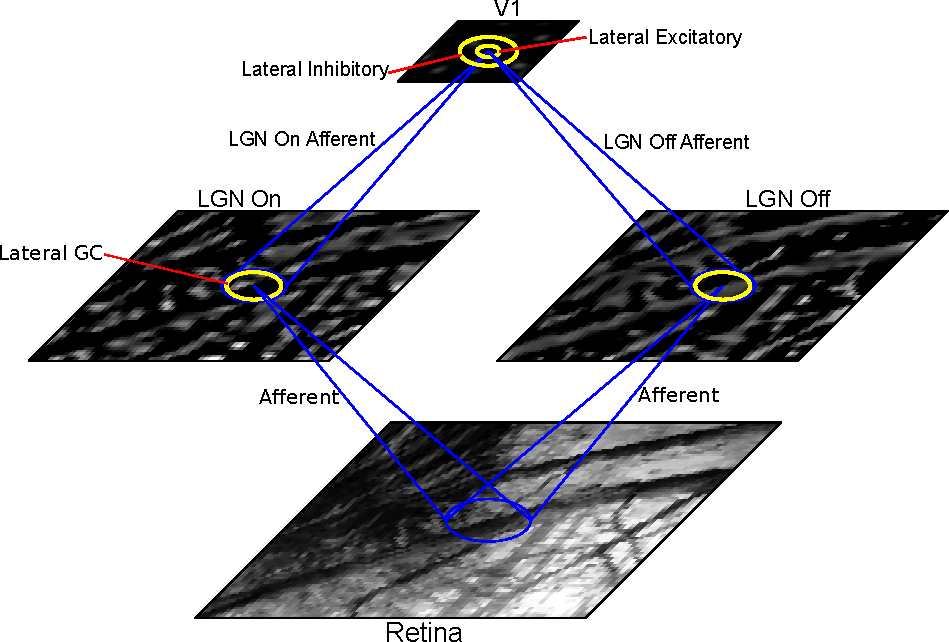
\includegraphics[width=1.0\textwidth]{GCAL.pdf}
	\caption[Schematic representation of the GCAL model. Reproduced
      from \cite{Stevens2013}.]{Schematic of simplest GCAL model for
      development of simple cells with surround modulation,
      retinotopic organization and orientation preference maps. It
      consists of a retinal sheet, two RGC/LGN sheets for ON and OFF cell
      responses and one V1 sheet, connected with intra- and
      inter-areal projections. The sheets are drawn to scale, with
      larger sheets for the RGC/LGN and retinal layers to avoid edge
      effects. Projections are illustrated with blue (feedforward
      connections) and yellow (lateral connections) ovals with cones
      converging on their target, all drawn to scale to show their
      spatial extents. RGC/LGN sheets consist of units with hardwired
      Difference of Gaussian RFs with ON and OFF center-surround
      regions. LGN Afferent projections to V1 are initially unspecific
      but develop Gabor-like RF structures through Hebbian learning of
      visual inputs, as observed experimentally. Reproduced from
      \cite{Stevens2013}.}
	\label{GCAL}
\end{figure}

The architecture of the GCAL model in its simplest form and as it will
initially be used in this project relies on only four sets of neurons
organized into 2D grids, which will be referred to as sheets. These
sheets consist of the retinal sheet for the presentation of stimuli,
two RGC/LGN sheets representing ON and OFF center receptive fields and
a V1 sheet. Neurons in these layers are connected with different
intra- and inter-areal connection fields. This simple model can only
be used to demonstrate retinotopy, orientation preference and the
emergence of simple cell-like RFs, but more complex models have been
shown to additionally account for complex cells, ocular dominance,
motion direction, spatial frequency, temporal frequency, disparity and
color \citep{Bednar2012a}. All these models are trained by presenting
a visual input on the retina, allowing the response to propagate
through the different sheets and then adjusting the connections
weights to V1 neurons based on a local learning rule.

This limited number of mechanisms already gives rise to an incredibly
robust model of development of topographic map development and
generates different experimentally observed RF profiles. To add
further robustness to the LISSOM model and to allow it to respond
across a wide range of contrasts, in GCAL contrast-gain control was
introduced in the LGN sheets (marked as Lateral GC). This mechanism
was closely modeled on the divisive normalization model introduced and
validated by \cite{Bonin2005}. Finally, the lateral excitatory and
inhibitory fields in the V1 sheet give rise not only to the
topographic map structure but also to some limited surround-modulation
effects.

Indeed there are existing models based on this architecture designed
to account for both complex cells and surround modulation
\cite{Antolik2010}. This model mirrors the approach taken in this
thesis in some ways, however modeling complex cells adds significant
additional computational overhead and makes it more difficult to
reason about the roles of different inhibitory
components. Additionally, the model is only coarsely spatially
calibrated making it more difficult about the precise extents of
individual connections. The major real difference is in the profile of
activation of inhibitory neurons, as excitatory neurons activate
inhibitory cells in a larger radius than other excitatory cells, while
the models here assume that excitatory cells project over the same
distance and it is the the inhibitory neurons that target a larger
area, mirroring the properties of large basket cells. Finally it is
not quite clear to what extent the model exhibits long-range
facilitation. However, the model should be seen as complementary to
the models that will be introduced in this thesis and may be combined
in future.

Overall, due to the simplicity of its mechanisms and its explanatory
strength, GCAL provides an ideal starting point to explore the
contribution of feedforward and lateral components to the response and
function of V1. Most importantly it provides an alternative to
static models of the visual cortex, which are unconstrained by the
requirement of having to developing into a functional circuit that can
actually capture features of the visual input. Therefore the GCAL
model sits at the three-way intersection between anatomical
organization, circuit-level and algorithmic implementation, and the
actual functional consequences on the response and computation
performed by this brain area. However, while existing models have
focused on the overall principles of self-organization, they have not
been used to study specific interactions between cell classes, how
those contribute to development and how the cortical circuit can adapt
to the specific computational requirements driven by a task.  These
topics will be the focus of the remaining chapters.
